\documentclass{uvamscse}
\usepackage{placeins}

\usepackage{listings}
\usepackage{xcolor}

\lstdefinelanguage{sdf}{%
  numbers=none,
  morekeywords={module,imports,exports,sorts,context,lexical,free,syntax,==,=,+,-,left,cons,prefer,avoid,bracket},
  columns=flexible,
  morestring=[b]",
  basicstyle=\footnotesize\mdseries,
  literate={->}{{\,\,$\to$\,\,}}1
}

\definecolor{colorRascalKeyword}{RGB}{106,63,96}
\definecolor{colorRascalString}{RGB}{176,133,155}
%\definecolor{colorRascalString}{RGB}{2,112,10}
\definecolor{colorRascalComment}{RGB}{150,152,150}

\lstdefinelanguage{rascal}{
  morekeywords={syntax, keyword, lexical, break, continue, finally, private, fail, filter, if, tag, extend, append, non-assoc, assoc, test, anno, layout, data, join, it, bracket, in, import, all, solve, try, catch, notin, else, insert, switch, return, case, while, throws, visit, for, assert, default, map, alias, any, module, mod, public, one, throw, start, value, loc, node, num, type, bag, int, rat, rel, lrel, real, tuple, str, bool, void, datetime, set, map, list},
  morestring=[b]",
  basicstyle=\footnotesize\mdseries,
  keywordstyle=\color{colorRascalKeyword}\bfseries\rmfamily,
  stringstyle=\color{colorRascalString}\ttfamily,
  commentstyle=\color{colorRascalComment}\ttfamily,
  morecomment=[l][\color{colorRascalComment}]{\//}
}

% Same colors in Rebel (Rascal colors)
\lstdefinelanguage{rebel}{
  morekeywords={module, import, specification, fields, events, event, lifeCycle, initial, final, new, this, preconditions, postconditions, function},
  morestring=[b]",
  basicstyle=\footnotesize\mdseries,
  keywordstyle=\color{colorRascalKeyword}\bfseries\rmfamily,
  stringstyle=\color{colorRascalString}\ttfamily,
  commentstyle=\color{colorRascalComment}\ttfamily,
  morecomment=[l][\color{colorRascalComment}]{\//},
  morecomment=[l][\color{colorRascalComment}]{@}
}

% Source: https://tex.stackexchange.com/questions/47175/scala-support-in-listings-package
% Missing colors
\lstdefinelanguage{scala}{
  morekeywords={abstract,case,catch,class,def,%
    do,else,extends,false,final,finally,%
    for,if,implicit,import,match,mixin,%
    new,null,object,override,package,%
    private,protected,requires,return,sealed,%
    super,this,throw,trait,true,try,%
    type,val,var,while,with,yield},
  otherkeywords={=>,<-,<\%,<:,>:,\#,@},
  sensitive=true,
  morecomment=[l]{//},
  morecomment=[n]{/*}{*/},
  morestring=[b]",
  morestring=[b]',
  morestring=[b]"""
}

\lstdefinelanguage{log}{
  %morekeywords={},
  %morecomment=[l]{//},
  %morestring=[b]",
}

\lstset{%
  frame=none,
  xleftmargin=2pt,
  stepnumber=1,
  numbers=left,
  numbersep=7pt,
  numberstyle=\ttfamily\scriptsize\color[gray]{0.3},
  belowcaptionskip=\bigskipamount,
  captionpos=b,
  tabsize=2,
  emphstyle={\bf},
  stringstyle=\itshape,
  showspaces=false,
  keywordstyle=\bfseries\rmfamily,
  columns=flexible,
  basicstyle=\small\ttfamily,
  showstringspaces=false,
  breaklines=true, % sets automatic line breaking
}


% % % % % % % % % % % % % % % % % % % % % % % % % % % % % % % %
% New commands
\newcommand{\cmd}[1]{\texttt{$\backslash$#1}}
\definecolor{codegray}{gray}{0.9}
\newcommand{\code}[1]{\colorbox{codegray}{\texttt{#1}}}
%\newcommand{\code}[1]{\texttt{\leavevmode\unskip $`$#1$`$}}
%\PackageWarning{TODO:}{Remove todos on final!!!}
%\newcommand\todo[1]{{\marginpar{\textcolor{red}{$-$ TODO:\\#1}}}}
%\renewcommand\todo[1]{} % Turns off all TODO's
\newcommand\pinfo[1]{{\marginpar{\begin{flushleft}\textcolor{blue}{|\\#1}\end{flushleft}}}} %  Left align in \pinfo's with "flushleft"
\renewcommand\pinfo[1]{} % Turns off all \pinfo's

% % % % % % % % % % % % % % % % % % % % % % % % % % % % % % % %
% Customization
\usepackage{fancyhdr} % Fancy header package
\pagestyle{fancy} % Enable
\fancyhf{} % Clear
\fancyhead[L]{\leftmark} % Fancy header
\fancyfoot[C]{\thepage} % Leave page numbers on footer

\def\chapterautorefname{Chapter} % "Chapter X" instead of "SS X" when referring to chapters
\def\subsectionautorefname{Subsection} % "Subsection X" instead of "SS X" when referring to subsections
\renewcommand{\arraystretch}{1.3} % Vertical spacing in tables
\usepackage[labelfont=bf]{caption} % Make figure and table tags bold too

% % % % % % % % % % % % % % % % % % % % % % % % % % % % % % % %
% Front matters

\title{ATUR: Automated Testing Using Rebel}
% \coverpic[100pt]{figures/terminal.png}
%\subtitle{Automatically testing a generated system using its input language}
\subtitle{Testing a generator using its input language and output system}
% \date{Spring 2014}

\author{Alex Kok}
\authemail{alexkok08@gmail.com}
\supervisor{Jurgen J. Vinju}
\hostsupervisor{Jorryt-Jan Dijkstra}
\host{ING, \url{http://www.ing.nl}}

% % % % % % % % % % % % % % % % % % % % % % % % % % % % % % % %
% Content
% Research questions

% RQ Main \ How can we automatically test the implementation of the generated program?

  %\item Which of the existing approaches best fits our situation to determine the test cases? \info{(Which properties of Rebel should be tested and how are these defined?)}
 % RQ 1 \item How can we automatically generate the tests, such that it can test a part of the generated system?
  % - Properties
  % - Define in Rebel > Translate to Scala with generator > Scala tests > Run
 % RQ 2 \item What kind of errors can we find using this approach?
  % - Implementation of operations, such as equality, addition, multiplication, etc.
  % - Precision errors? (is basically the above?)
  % RQ 3 \item How can we extend our test suite to find more implementation errors?
  % - Add sync block
  % - Even more properties, but should be useful ones

% Old one
%\def \rqMain{ How can we automatically test the implementation of a component in the generated system against the Rebel specification, to check whether the implementation works as expected? }
% New
% Or something like:
% - Wat zegt het gegenereerde systeem over de kwaliteit van de generator mbt Rebel types?
% -
\def \rqMain{
	How can we automatically test the generator in the \textit{Rebel} toolchain, by using the generated system, to check whether the implementation works as expected?
}
% Old one: Too vague, PBT wasn't mentioned, so 'automatically' was also unclear
% \def \rqOne{ How can we automatically generate the tests, such that it can test a component the generated system? }
% New
\def \rqOne{
	Which properties are expected to hold on the semantics of the generated code?
}
% Old one: zoom in, # of bugs and which type?
%\def \rqTwo{ What kind of errors can we find using this approach? }
% New
\def \rqTwo{
	How can we test each property as automatically as possible to find bugs in the generator?
}
% Old one: future work question...
%\def \rqThree{ How can we extend the test suite to find more implementation errors in the generated system? }
\def \rqThree{
	What kind of bugs can be found using this approach and how many?
}

% % % % % % % % % % % % % % % % % % % % % % % % % % % % % % % % % % % % %
% Abstract?
\listoftodos[Todo's]
% % % % % % % % % % % % % % % % % % % % % % % % % % % % % % % % % % % % %
% Chapter: Introduction
% % % % % % % % % % % % % % % % % % % % % % % % % % % % % % % % % % % % %
\chapter{Introduction}
\label{chp:intro}
\pinfo{Short about Rebel}
Large systems often suffer from domain knowledge that is implicit, incomplete, out of date or ambiguous definitions. This is what \textit{Rebel} aims to solve \cite{stoel2016solving}. The toolchain of \textit{Rebel} can be used to check, simulate and visualize the specifications, allowing to reason about the final product \cite{stoelcase}. Checking is done based on bounded model checking by using the Z3 solver.\\
\\
\pinfo{Aim of project}
Generators are being used to generates a system from the Rebel specifications. The generated system provides an API interface in order to work with the specified product and handles the database connectivity. However, the implementation of the generated program is not checked against the specifications, meaning that the generated program is perhaps not doing what it is supposed to do according to its specifications. The aim of this project is to improve this, by automatically testing the generated program against Rebel specifications.

% % % % % % % % % % % % % % % % % % % % % % % % % % % % % % % % % % % % %
% Section: Initial study
% // Don't think it's needed? Rebel papers?
% // It's in background too, about Rebel and what Rebel does.

% % % % % % % % % % % % % % % % % % % % % % % % % % % % % % % % % % % % %
% Section: Problem statement
\section{Problem statement}
\pinfo{Translation from generator and why automatically}
From the \textit{Rebel} specifications, a system can be generated by the generator. However, neither the generator, nor the generated program is being tested against the specification. Thus it could be that the generated system doesn't work according to what is specified in the \textit{Rebel} specification. Although the generator should translate everything correctly, we cannot assume that it actually does translate it correctly for each case and that the implementation works as expected.\\
\\
Currently, there are no tests for the generator or the generated system, during the development of the generator the results are being checked manually. Testing is a major cost factor in Software Development, with test automation being proposed as one of the solutions to reduce these costs \cite{ramler2006economic}. We aim for an approach such that much of the testing is automated to reduce the time (and costs) needed for testing certain components of the generated system.\\
\\
The main research question is as follows:
\begin{quote}
  \rqMain
\end{quote}
We investigate the following solution: generating tests based on a \textit{Rebel} specification and then run these tests against the generated system.\\
\\
% - Property based testing is a possible path, which we will do.
\pinfo{Possibility: PBT + short explanation}
Property-based testing is an approach to validate whether an implementation satisfies its specification~\cite{fink1997property}. It describes what the program should or should not do. As~\cite{fink1997property} describes: ``Property-based testing validates that the final product is free of specific flaws.". With property-based testing, a property is being defined which should hold on the system. Next, the property is being tested for a certain amount of tries, using different input values to check whether the property holds. In case the property doesn't hold, it will result in a failure, reporting that there is a case in which the property doesn't hold. Indicating that a bug in the system has been triggered.\\
\\
\pinfo{Doing it too, worked already on x, x and x}
Property-based testing has already shown a success in earlier studies~\cite{fink1997property,claessen2011quickcheck,arts2006testing}, detecting errors in a system that were not known before. In this thesis we will use property-based testing to check the generator, using the generated system to check whether the properties hold.\\
\\
% - Hypothesis? We will find bugs in the generated system using this approach. Although errors could have been found (and fixed) already by manual testing/checking and code reviews,  we expect to detect yet unknown bugs in the generated system.
\pinfo{Hypothesis, we will detect}
We hypothesize that there are yet unknown bugs in the generator, resulting in that the generated system does not work as expected. By using property-based testing we expect to detect bugs in the generator.\\
\\
To answer the main research question, we will first answer the following research questions:
\begin{description}
\item[~~~~RQ 1:] \rqOne
\item[~~~~RQ 2:] \rqTwo
\item[~~~~RQ 3:] \rqThree
\end{description}

% - Shortly describe how this is done, and how it would find bugs, test mechanics explain it in more detail, image in test mechanics.
\pinfo{In short: how. Details are in CH3}
\todo{Is this needed here? Maybe remove or place somewhere else?}
The generator takes a \textit{Rebel} specification as input. Which contains the properties that are expected to hold in the generated system. Next, \textit{Scala} tests are being generated based on the properties, using the existing generator to translate the expressions used in the properties. These tests will be run against the generated system, to check whether each property holds. In case a test of a failing test, a bug has been found. There are multiple generators available within ING. Throughout this thesis, we will use the most mature generator, which is the Scala/Akka generator. This generator is often used for other experiments too.\\
\\
\pinfo{Assumptions}
In order to run the test suit, we assume that the generated system can be compiled and that it can be run. Furthermore, the specification which was used to generate the system should be syntactically and semantically correct. Which means that the \textit{Rebel} type checker should not report any error about the specification.\\
\\
\pinfo{Not detecting everything, but checking properties}
The test framework generates a test suite that can be run against the generated system. In case the test suite finishes without errors, it means that it did not found any bugs and that the generator satisfies the properties that were tested. This doesn't mean that there are no bugs in the generated system, instead, it means that our test suite was not able to find errors in the properties that it checks for. The generated system will probably still contain bugs which are not detected by using the test framework. In this case, improving the test framework might extend the number of bugs that it can find.

% % % % % % % % % % % % % % % % % % % % % % % % % % % % % % % % % % % % %
% Section: Research method
\section{Research method}
% In short, describe steps:
% // (Steps also interesting for mechanics chapter)
% 1 Defining properties, define what is unknown yet and what it actually means.
% 2 Describe how tests can be generated out of this. From these properties to Scala tests. (Properties > Rebel events > Scala tests per event, with random values)
% 3 Describe how we measure our experiments
% 4 Evaluate the results. Can we reason about it? What have we covered and also what have we not covered?
\pinfo{First defining properties, then small example}
We will start off with defining the properties that are expected to hold on the generator. Then we describe how these properties can be tested on the generator, using one property to demonstrate the working of the test framework. We can then run the tests suit against the generated system and check if this method actually works to detect bugs.\\
\\
\pinfo{Generate, run, evaluate results and improve again}
Next, we generate tests for each of these properties and run these against the generated system. After running the test suit, the result is being evaluated. When one or more tests are failing, a bug is found. However, we need to investigate the failing case such that we discover what the actual bug is. After evaluating we improve our test generation and continue to evaluate the results again.

% % % % % % % % % % % % % % % % % % % % % % % % % % % % % % % % % % % % %
% Section: Contribution
\section{Contribution}
% - Definitions (properties)
% Before, in conclusion:
% We provided a definition of some types in \textit{Rebel} and described properties that should hold when using operations with these types. Since there were no clear definitions available yet of what these types exactly do, a contribution has been made to the \textit{Rebel} project, such that there are now some definitions and properties available. This also helps when reasoning about the implementation, as there is now a definition of what is expected. Although these definitions might change over time, it allows to reason back to an earlier starting point.\\
We provide definitions of the properties that are expected to hold when using the \textit{Rebel} language and its toolchain. Allowing to reason about the generator and whether the implementation satisfies these properties. There are no property definitions of \textit{Rebel} yet, so we provide a starting point for this with the focus on the important properties.\\
\\
% - A way to automatically test the generator and generated system using Rebel, defining properties as events
% Before, in conclusion:
% We have shown a way to automatically test the generator using the \textit{Rebel} language and its toolchain, with the addition of our test framework. This is done by defining the properties that are expected to hold in the first case. Which can be translated to a \textit{Rebel} specification such that a system can be generated from it. Additionally using the generator when generating the test cases, so that the translation of expressions in the generator will be checked too. The different kind of properties should be able to detect unexpected behaviour.\\
The defined properties are being used to check the generator. We come with a solution that uses the input that is required for the generator and the output of the generator to check the generator. This process should be as automatic as possible, such that it doesn't require much time to make use of it. Our test framework will combine the required steps to detect bugs as automatically as possible.\\
\\
% - Found number of bugs in generated system
% Before, in conclusion:
%A number of bugs have been found in the generated system, precision errors, overflow/underflow errors and even a compile error. These bugs are now known issues in this project, while these were unknown before. This shows us that this approach already worked in such a way that it is able to detect bugs in the generated system. It can be extended to detect even more bugs. With some modifications, it is also possible to use this approach with other generated systems, such that it can detect inequalities among these.\\
The generator that is being used is expected to contain bugs. Therefore, we expect to detect, yet unknown, bugs in the generator. These bugs are then known bugs and can be fixed. The bugs found will then also indicate what kind of bugs we can detect in a generator by using this approach.

% - Squants issues
% Before, in conclusion:
%In this approach, we identified two bugs, which were due to an open-source library used in the generated system, called \textit{Squants}. We reported these two issues, such that these can be fixed in a later version of the library.

% % % % % % % % % % % % % % % % % % % % % % % % % % % % % % % % % % % % %
% Section: Related work
\section{Related work}
% // Doesn't this have to be at the end?
% - Testing of (extended) finite state machines

% % % % % % % % % % % % % % % % % % % % % % % % % % % % % % % % % % % % %
% Subsection: Random testing
\subsection{Random testing}
\pinfo{Describe random testing (FDRT)}
Random testing is a technique in which random values are being used as input for the test cases. \textit{QuickCheck} \cite{claessen2011quickcheck} and \textit{Randoop} \cite{pacheco2007randoop} are examples of random testing techniques. These differ in how they automatically test systems and what actually is being tested. QuickCheck is based on property-based testing, which we also apply in this project. \textit{Randoop} on the other hand is based on feedback-directed random testing.\\
\\
\pinfo{Describe FDRT}
With feedback-directed random testing, random tests are generated which will immediately be run. The result of earlier test attempts can affect the next test that is being generated, which can be seen as feedback for the next generated test. This allows each test case to 'learn' from earlier attempts and to create unique tests.\\
\\
\pinfo{About Randoop, shortly how it works}
\textit{Randoop} is build for Java projects and checks some built-in specifications of Java that can't be checked by the compiler. The test cases are simple unit tests, consisting of a unique sequence of methods due to the feedback of earlier attempts. The method sequences are unique because it also checks whether the same case has already been checked. Since there can be unlimited sequences of methods to test, the test suite will be terminated after a defined timeout. Next, the result is determined and failing cases are being reported, although when using this approach it cannot determine whether the whole system is correct according to the Java specifications. Instead, it just wasn't able to find a case for which it fails. This is a useful approach to generate unique tests, but its goal is to check systems built in Java and thus is not compatible with the semantics of Rebel. It works with calling the Java objects and using methods on those, while the generated system consists of mainly states and events. When using an approach like \textit{Randoop} with random input values, it cannot be known whether the result of a specific transition was expected to succeed or fail.\\
% Can add DART here, if needed
\\
\pinfo{Our case, why existing approaches can't be used}
%  Background contains info about quickcheck and randoop. Repeat limitations and describe how we do it
Approaches like \textit{QuickCheck} \cite{claessen2011quickcheck} and \textit{Randoop} \cite{pacheco2007randoop} enforce the system under test to be written in a specific language (\textit{Haskell} for \textit{QuickCheck}, \textit{Java} for \textit{Randoop}). For \textit{QuickCheck} there are alternative solutions for other languages. In our case, we need to use \textit{Rebel} when generating test cases, such that we test the generator when generating the tests. Another reason why we can't use a method like \textit{Randoop} is that \textit{Randoop} strictly checks for \textit{Java} properties, which are not in line with the \textit{Rebel} language.

% % % % % % % % % % % % % % % % % % % % % % % % % % % % % % % % % % % % %
% Section: Outline
\section{Outline}
\todo[inline]{Write later, when outline is more final.}
% 1. Describing background
% 2. Defining properties
% 3. Test mechanics
% 4. Experiment 1
% 5. Experiment 2
% 6. Conclusion
% 7. Threats of validity
% 8. Future work?

% % % % % % % % % % % % % % % % % % % % % % % % % % % % % % % % % % % % %
% Chapter: Background and context
% % % % % % % % % % % % % % % % % % % % % % % % % % % % % % % % % % % % %
\chapter{Background and context}
\label{chp:background_and_context}
% % % % % % % % % % % % % % % % % % % % % % % % % % % % % % % % % % % % %
% Section: Rascal
%\section{Rascal}
% // Not explaining Rascal for now
% - Rascal is a Meta-progrmaming language which is used throughout the project.
% - Rebel is written in Rascal.\\
% - The generators are also written in Rascal.\\
% - Our test generator is also written in Rascal. However, the resulting tests are written in Scala.

% % % % % % % % % % % % % % % % % % % % % % % % % % % % % % % % % % % % %
% Section: Rebel
\section{Rebel}
\pinfo{About Rebel}
\textit{Rebel} is a domain specific language that focuses on the banking
industry~\cite{stoel2016solving}. Banking products can be specified in the
language, with the use of types like \textit{Money} and \textit{IBAN}. The tool
chain of \textit{Rebel} allows to check, visualize and simulate the specified
banking product. For checking and simulation an efficient, state-of-the-art SMT
solver is being used called \textit{Z3}, which is developed by
\textit{Microsoft}~\cite{de2008z3}. \textit{Rebel} is written in \textit{Rascal}
and is developed by the \textit{ING} in corporation with the \textit{CWI}.
Currently, the tool chain of \textit{Rebel} is also written in
\textit{Rascal}.\\
\\
\pinfo{What Rebel exactly checks}
Checking a \textit{Rebel} specification is based on Bounded Model
Checking~\cite{stoel2016solving}. The \textit{Rebel} specification is being
translated to SMT constraints, next, the \textit{Z3} solver is being used to
check whether the specification is consistent. An inconsistent specification
means that a counter example has been found (meaning that a trace is found for which an
invariant doesn't hold). It is bounded since it only checks if a counter example
can be found within a certain number of steps. Besides checking the
specification, the specification can also be simulated. For simulation, the SMT
solver is also being used to determine whether a transition can happen. After
successfully checking the specification, meaning that no counter examples could
be found, the result is still that the specification `might' be valid. As the
checking method is bounded, it stops at a certain point (which, in the
\textit{Rebel} toolchain, is defined as the maximum depth of the traces that can
be used for checking). This means that there can still be a long or untested
trace for which the invariant doesn't hold.\\
\\
\pinfo{Generating system from specification}
From the \textit{Rebel} specification, a system can be generated by using a
generator which is developed by \textit{ING}. The generators are also written in
\textit{Rascal}. This requires a specification that is consistent and that does
not trigger errors by the type checker. Although the specification is being
checked by using bounded model checking, the generated system is not being
checked against the specification. Unfortunately, it is not possible to also use
the bounded model checker to test the generator or the generated system. As the
generated system is written in \textit{Scala}, while the existing checker only
supports checking the \textit{Rebel} specification itself.

% % % % % % % % % % % % % % % % % % % % % % % % % % % % % % % % % % % % %
% Section: The Scala/Akka generator
\section{The Scala/Akka generator}
% Generator -> Scala, Akka, test config missing in prototype, thus we add that ourselves. Using Doubles for Percentage. Might expect problems on here. Known problems with Doubles etc.
\pinfo{Different generators, we use Scala/Akka generator}
There are multiple generators developed within \textit{ING}. The generators are
different in that the resulting product is written in a different language or
uses a different implementation, like database or messaging layer. Each
generator is written in \textit{Rascal}. \textit{Rebel} defines the states and
the transitions between the states in the \textit{lifeCycle} block, which can be
seen as the Finite State Machine definition of the specified product. The
Scala/Akka generator is one of these generators. It generates a system that is
written in \textit{Scala}, uses \textit{Akka}~\cite{siteAkka2017} as actor
system and uses \textit{Cassandra}~\cite{siteCassandra2016} as database. A resulting
system of this generator is also tested thoroughly with performance tests, to
reason about how well this system performs with its architecture. However, this
does not check the implementation of the generated system against the
\textit{Rebel} specification. This generator is often used within experiments
inside \textit{ING} and is considered the most mature generator among the
currently developed generators. Because of this, it's interesting if we
encounter yet unknown problems in the generator itself or the resulting system.
Throughout this thesis, we will only make use of this generator.\\
\\
\pinfo{Short explanation on implementation generated system + why}
A specification can be defined in terms of a Labeled Transition
System~\cite{stoel2016solving}%\todo{SRC-Rebel-Reference on smt check chapter. Do we need that source? ("As introduced by Keller 1876") Just citing Rebel is probably OK too}
, containing the states, the data fields and the transitions between the states
along with the pre- and post conditions of the transitions. The generated system
is based on these states and transitions defined in \textit{Rebel}, resulting in
a system that works like an Extended Finite State Machine. Thus the generated program
also implements it like states and transitions between them. An instance of a
banking product can have fields and is in a specific state. In order to go to
another state, a transition can be done which might have pre- or post conditions.
In case there are pre- or post conditions, these have to be satisfied in order to
successfully complete a transition.\\
\\
\pinfo{Diff types: known/expected problems. We have to specify expected properties}
\textit{Rebel} introduces custom types, such as \textit{IBAN},
\textit{Percentage} and \textit{Money}, these types are not supported natively
in \textit{Scala}. For these cases, a library or own implementation is used. An
example is the \textit{Money} type, which is available in the
\textit{Squants}~\cite{siteSquants2017} library. The generated system uses this
library to deal with the \textit{Money} type and its operations. Another example
is the \textit{Percentage} type, which is simply translated by calling a method
\code{percentage()}. In order to conclude that the generated program is doing
something incorrectly, we have to specify what the expected properties are in
\textit{Rebel}.


% % % % % % % % % % % % % % % % % % % % % % % % % % % % % % % % % % % % %
% Section: Property-based testing
\section{Property-based testing}
\pinfo{About property-based testing}
With property-based testing properties are defined and being tested. It uses random values as input and checks whether the defined property holds. After a certain number of succeeding cases the test succeeds and the next property is being checked.\\
\\
\pinfo{About QuickCheck}
A well-known tool which is based on property-based testing is
\textit{QuickCheck}, which is written for
\textit{Haskell}~\cite{claessen2011quickcheck}. It tests the properties
automatically by using random input values. For each property
\textit{QuickCheck} tries to find counter examples, which are a set of values
for which the desired property does not hold. If 100 test cases are succeeding
in a row, it goes on to the next property. In case it found a counter example,
it will try to minimize the values to try to report the edge case of the
failure. However, one might have properties that only hold under certain
conditions. For this \textit{QuickCheck} allows using preconditions. Although,
this doesn't work well for every case as \textit{QuickCheck} will just generate
new pairs of values in case the precondition didn't hold for the generated set
of values. An example of this is where 2 of the input values have to be equal,
the chance that this happens with random values is rather low.
\textit{QuickCheck} will try to generate new values each time, with a maximum of
1000 tries by default. In case this maximum is reached, it reports the case as
``untested'' and continues to the next property. Note that these values of 100 and
1000 are the default values, these can be adjusted when needed.\\
\\
\pinfo{About the ports of it}
% Different ports, for example FortressCheck
Due to the effectiveness of \textit{QuickCheck}, many ports for other languages
were written. Most ports implement the basics of \textit{QuickCheck},
additionally, each port could have added extra features. Examples of some ports
are \textit{FortressCheck} (for \textit{Fortran})~\cite{kang2011fortresscheck}
and \textit{ScalaCheck} (for \textit{Scala})~\cite{siteScalaCheck2015}.
\textit{FortressCheck} supports polymorphic types and, unlike
\textit{QuickCheck}, heavily uses reflection for its value generation to solve
certain problems with polymorphic constructs. Although \textit{Scala} supports
polymorphism, \textit{ScalaCheck} does not use reflection to test
this~\cite{kang2011fortresscheck}.\\
\\
\pinfo{No QuickCheck for Rebel, not using ScalaCheck}
There is no \textit{QuickCheck} implementation for \textit{Rebel}. As the
generated system is written in \textit{Scala}, \textit{ScalaCheck} might be
applicable for us. However, this would result in using \textit{ScalaCheck} as a
black box, implementing the random functionality ourselves makes sure we know
what is going on. Thus resulting in a white box implementation for our test
framework.\\
\\
\pinfo{Custom modifications}
We can also modify it to our needs when we want to improve our test suite. One
of the things that we want to improve is to generate values under certain
conditions. For example, if a property only holds under a certain condition, the
chance that random values satisfy the condition can be very low. Resulting in a
test case that wouldn't do anything most of the time. An example of such a
property is \textit{Symmetry} (\code{x == y $\implies$ y == x}). %, which defines that y should be equal to x iff x is equal to y.
Additionally, we might also need to slightly interact with other components,
such as the messaging layer, that the generated system uses. This could make the
implementation more complicated when using \textit{ScalaCheck} due to the format
of a property test when using \textit{ScalaCheck}.

% % % % % % % % % % % % % % % % % % % % % % % % % % % % % % % % % % % % %
% Section: Terminology
\section{Terminology}
\pinfo{Confusing terminologies and abstractions}
In this thesis there are some levels of abstraction, the terminology used
throughout this theses can cause confusion. Words like `specification',
`properties' and `tests' generally can have a different meaning depending on the
context. In this section, we describe the confusing terminologies and
abstractions in detail.

\begin{description}
\item[Specification]\hfill\\
In this thesis we use the word ``specification'' exclusively to indicate
banking products described in the \textit{Rebel} language. This includes the
state machines (life cycle), pre and post-conditions and logical invariants.

\item[Properties]\hfill\\
We use the word ``property'' to describe semantic properties of the
\textit{Rebel} language. The set of properties we introduce in this thesis can
be seen as a partial ``specification'' of the semantics of \textit{Rebel}, but
we do not use this word to avoid confusion. We stick with ``properties''.

\item[Implicative property]\hfill\\
A ``property'' that uses the implication ($\implies$) operator in its
definition.

\item[Generator(s)]\hfill\\
The generator(s) that can be used to generate a system based on a
``specification''. When using the term ``the generator'', we refer to the
Scala/Akka generator which is the only generator that we use throughout this
thesis.

\item[Test framework]\hfill\\
The test framework that was developed during this thesis. Which builds the
specification, generates a system from the specification by using the generator,
generates the test suite and runs the test suite against the generated system.

%\item[System Under Test (SUT)]\hfill\\
%The system against which the tests are being run. This system is generated by using a generator. Also referred to as ``generated system'' in the context of generating the ``system under test''.

\item[Tests]\hfill\\
The generated tests by the ``test framework'', intended to check whether a
certain ``property'' holds.

\item[Test suite]\hfill\\
The collection of generated tests by the ``test framework'', along with its configurations which can
be run to test the generated system. Note that the test suite initially doesn't
exist. Instead, it is being generated and added to ``the generated system'' when
we run the ``test framework''.

\item[Events]\hfill\\
The event definitions in a ``specification'', these define the transitions
between the states.

\item[Scala Build Tool (SBT)]\hfill\\
The tool that is used to compile and run the ``generated system'' and the
``test suite''.

\item[Concrete Syntax Tree (CST)]\hfill\\
A ``specification'' can be checked and built. This results in a ``CST''
containing the data of the specification. This ``CST'' is being used by the
toolchain of \textit{Rebel} and by the ``test framework''.

% Common knowledge, right? :
%\item[Invariant(s):]\hfill\\
%The invariant of a \textit{Rebel} specification defines conditions that should always hold during the life cycle of an instance of the product.
%\item[Read–Eval–Print Loop (REPL)]\hfill\\
%...
%\item[Application Programming Interface (API)]\hfill\\
%...
\end{description}

% % % % % % % % % % % % % % % % % % % % % % % % % % % % % % % % % % % % %
% Chapter: Property definitions
% % % % % % % % % % % % % % % % % % % % % % % % % % % % % % % % % % % % %
\chapter{Properties of Rebel}
\label{cpt:properties}
% Definition: An Axiom is a mathematical statement that is assumed to be true.
% ( http://www.aaaknow.com/lessonFull.php?slug=propsCommAssoc )
% Sources:
% Axioms in algebra — where did they come from?
% http://www.jstor.org.proxy.uba.uva.nl:2048/stable/pdf/27956337.pdf?refreqid=excelsior%3A623b1c85f79f8cd18bc9d09560339b9b
% (simple formulas, history, and explanations)
% A perspective on the algebra of logic
% http://www-tandfonline-com.proxy.uba.uva.nl:2048/doi/pdf/10.2989/16073606.2011.622856?needAccess=true
% (More formulas, deeper explanations)
% Might contain more properties

% Another source was (but not a paper or so)
% http://www.aaamath.com/ac22.htm

% Another good source (book)
% Calculus, Vol. 1: One-Variable Calculus, with an Introduction to Linear Algebra 2nd Edition

\pinfo{Specific types in Rebel}
Rebel introduces specific types, like \textit{Iban} and \textit{Money} and
allows operations on those~\cite{stoel2016solving}. But what are the expected
properties of the generator? In this chapter we will try to answer the first
research question:
\begin{description}
	\item [~~~~RQ 1:] \rqOne
\end{description}
To answer this question, we first describe a way how we can determine the
properties. Followed by the property defintions that will be used troughout this
thesis, with a motivation why these properties are expected to hold.

%\todo[inline]{Percentage? Not yet, defining those requires properties again. And running the test suit again, evaluate again, etc.\\
%Describe what exactly is Percentage if we define it in a specification, which rules does it inherit?\\
%Percentage (expected): 2/more decimals, however its a precise amount. Calculating with it is expected in a result of the real value.\\
%Percentage (current): As it is defined now: full number, it can exceed 100. However it does not support decimals yet.}

% % % % % % % % % % % % % % % % % % % % % % % % % % % % % % % % % % % % %
% Section: Determining the properties
\section{Determining the properties}
\pinfo{Properties not defined for Rebel. We must define these}
Currently, there are no definitions available of what the properties are of each
type and operation in \textit{Rebel}. Due to the missing definitions of these
types, it means that we first have to define what the the expected properties
on these types are and substantiate these. Only then we can determine whether
the generator is working as expected with these properties. As there are many
operations available among the available types in \textit{Rebel}, we are not
able to define all the properties that exist in the \textit{Rebel} language. As
there can be countless of properties and combinations among the different types
that \textit{Rebel} supports. During this thesis we will focus on the
\textit{Money} type, considering this is the most important type for a bank that
has the highest priority to be implemented correctly.\\
\\
\pinfo{Types and axioms}
For types like integers the axioms of algebra can be used to determine whether
the implementation in the generated system is correct. These are most likely
translated to integers in the generated system too, with perhaps the expectation
that these have the same properties in \textit{Scala}. However, it is not
possible to rely on the \textit{Integer} definition of a specific language, as
another generator might generate a system in another language, or might
implement it differently in the same language. Would that mean that the
properties on that other language should now hold on the \textit{Integer} type?
Well, as this is not defined for \textit{Rebel}, this is unknown. In this
chapter we will define properties that are expected to hold on the
\textit{Money} type in \textit{Rebel}. The properties that we define are based
on the known axioms in
algebra~\cite{baumgart1961axioms,raftery2011perspective,apostol2007calculus}.
We provide an explanation of why a certain property should also hold in these
cases.\\
\\
\pinfo{Amount, not floating-point arithmetic}
The \textit{Money} type can be seen as a currency with an amount value. The
amount of a \textit{Money} value can have multiple decimals depending on the
currency. Thus, the amount can be seen as a floating number. Does this mean that
it inherits the computation properties of Floating-Point Arithmetic, as defined
in the IEEE standards 754 or 854? Since the Rebel is intended to be a formal
specification language for banking products, we don't expect that the described
problems with this arithmetic are intended to exist on the Money type.
Considering that that a high volume flows within a bank in terms of
\textit{Money}, using the Floating-Point Arithmetic properties can result in the
known precision, overflow and underflow errors as described
in~\cite{goldberg1991every}. Such errors should be avoided when using the
\textit{Money} type. The author of \cite{fowler2002patterns} also describes that
the intend of the \textit{Money} type is to avoid this:
\begin{quote}
	``You should absolutely avoid any kind of floating point type, as that will
	introduce the kind of rounding problems that Money is intended to avoid.''
    -- Martin Fowler \cite{fowler2002patterns}
		%[p. 462] % Of pdf, ebook thing doesn't have page numbers
\end{quote}

\pinfo{Money operations, expecting division problem}
The author of~\cite{fowler2002patterns} also describes the operations that can
be done with the \textit{Money} type, which are: +, -, *, allocate, $<$, $>$,
$\leq$, $\geq$ and =. Where the allocate method is used instead of the
division~(/) operation. This is due to the division problem, requiring a number
to be rounded off at a certain time. For example, when splitting 1 EUR with 3
people, everyone would receive 33 cents, but what is done with the last cent
that is left? This is the problem that is being solved by the allocate method,
representing the ratio in which the rest amounts should be allocated (the last
cent would go to in this case)~\cite{fowler2002patterns}. The allocate method is
a thing that \textit{Rebel} does not have, instead it just allows the use of the
division operator. Because of this, we expect the division problem to occur
while running the test framework. The amount of a \textit{Money} value is often
rounded when it is being represented to the user, as it could have many
decimals. The representation of the \textit{Money} value is up to the business
on how this is done, as there are multiple factors influencing this. Instead, we
only focus on the internal value that is used when operating with the
\textit{Money} type.\\
\\
\pinfo{Not between different currencies}
It is unsupported to use these operations with \textit{Money} values when using
values that are of different currencies. This is this could be done by taking
the exchange rates into account, as described in~\cite{fowler2002patterns}.
However, this is not implemented in Rebel yet and thus it is unsupported to use
these operations when using different currencies.\\
\\
\pinfo{Equality, currency overrules}
When using equality both the currency and the amount are taken into account,
which should be equal for both variables. In case of different currencies, it is
not considered equal, even if the amount would be equal. \\
\\
\pinfo{Thus: precise value, rounding only for division}
We say that the amount of a \textit{Money} value in \textit{Rebel} should hold the exact value as if we would calculate the same expression by ourselves. Meaning that the precision errors would have to be prevented. An exception on this is when the result would be in the form of a fraction, for example 1/3. As this results in a value which we have to round up sometime. To fix this, we say that in this case we use x decimals when calculating, without rounding the x+1th decimal. When using properties with division, this should be taken into account in case the system fails on these tests. \todo{Define X, 4 decimals minimal?}

% % % % % % % % % % % % % % % % % % % % % % % % % % % % % % % % % % % % %
% Section: Property definitions
\section{Property definitions}
\label{sct:properties_property_definitions}
\pinfo{Properties based on known axioms, but has restrictions}
The properties that we define are based on the known axioms in algebra, although
not every property can be used.\\
\\
For example, it isn't possible to multiply two
\textit{Money} types with each other in order to support the multiplicative
property. This is becasue the type checker of \textit{Rebel} would not allow
multiplication between \textit{Money} types, additionally we should think of
what the result would be when two Money values are being multiplied. We consider
this as an unknown result type, thus it is reasonable that we cannot use
multiplication when using only \textit{Money} types. Division has a similar case
, as something cannot be divided a \textit{Money} type.\\
\\
Instead we can use these operations with \textit{Money} in combination with
other types, such as \textit{Integer} and \textit{Percentage}. The type checker
for \textit{Rebel} will be used to determine these combinations. Due to this,
one property definition can lead to different possible combinations which can be
used. This results in multiple property definitions when using different types.
In the following sections we motivate the properties that we use during the
project.
% % % % % % % % % % % % %
% Subsection: Reflexivity
\subsection*{Reflexivity}
% Table
\FloatBarrier
\begin{table}[!ht]
\centering
\begin{tabular}{lll}
\hline
                        \textbf{Formula} & \textbf{Property name} & \textbf{Variable (Type)} \\ \hline
\rowcolor[HTML]{EFEFEF} x == x           & reflexiveEquality      & x: Money                 \\
                        x $\leq$ x       & reflexiveInequalityLET & x: Money                 \\
\rowcolor[HTML]{EFEFEF} x $\geq$ x       & reflexiveInequalityGET & x: Money                 \\ \hline
\end{tabular}
\caption{Reflexivity when using \textit{Money}}
\label{tbl:ch4_money_reflexivity}
\end{table}
\FloatBarrier
% End table
% Reasoning
\pinfo{Equality, currency and amount}
The reflexive property means a relation of a type with
itself~\cite{raftery2011perspective}. An instance of type \textit{Money} should
be equal to itself. The inequality relations \textit{smaller or equal to} and
\textit{greater or equal to} should hold too, as we can compare \textit{Money}
variables. The equality relation exists on the \textit{Money} type, which is
also used in the first row of the table.

% % % % % % % % % % % % %
% Subsection: Symmetry
\subsection*{Symmetry}
% Table
\FloatBarrier
\begin{table}[!ht]
\centering
\begin{tabular}{lll}
\hline
                        \textbf{Formula}         & \textbf{Property name} & \textbf{Variable (Type)} \\ \hline
\rowcolor[HTML]{EFEFEF} x == y $\implies$ y == x & symmetric              & x: Money                 \\
\rowcolor[HTML]{EFEFEF}                          &                        & y: Money                 \\ \hline
\end{tabular}
\caption{Symmetry when using \textit{Money}}
\label{tbl:ch4_money_symmetry}
\end{table}
\FloatBarrier
% End table
% Reasoning
\pinfo{Equality, currency and amount}
Reflexivity already described equality on the same variable of the \textit{Money} type. When two different variables are used, the order should not matter and thus it should work in both ways. Which is known as the symmetric property~\cite{raftery2011perspective}.

% % % % % % % % % % % % %
% Subsection: Antisymmetry
\subsection*{Antisymmetry}
% Table
\FloatBarrier
\begin{table}[!ht]
\centering
\begin{tabular}{lll}
\hline
                        \textbf{Formula}                             & \textbf{Property name} & \textbf{Variable (Type)} \\ \hline
\rowcolor[HTML]{EFEFEF} x $\leq$ y \&\& y $\leq$ x $\implies$ x == y & antisymmetryLET        & x: Money                 \\
\rowcolor[HTML]{EFEFEF}                                              &                        & y: Money                 \\
                        x $\geq$ y \&\& y $\geq$ x $\implies$ x == y & antisymmetryGET        & x: Money                 \\
                                                                     &                        & y: Money                 \\ \hline
\end{tabular}
\caption{Antisymmetry when using \textit{Money}}
\label{tbl:ch4_money_antisymmetry}
\end{table}
\FloatBarrier
% End table
% Reasoning
The antisymmetric relation describes that whenever there is a relation from x to y and a relation from y to x, then x and y should be equal. The lower or equal then and greater or equal then relations fit in this category, as shown in \autoref{tbl:ch4_money_antisymmetry}. We can use these operations with the \textit{Money} type when both x and y use the same currency. This antisymmetric relation is also expected to hold, as \textit{Money} values should be equal when they are of the same currency and hold the same amount.

% % % % % % % % % % % % %
% Subsection: Commutativity
\subsection*{Commutativity}
\label{ssct:4_commutativity}
% Table
\FloatBarrier
\begin{table}[!ht]
\centering
\begin{tabular}{lll}
\hline
                        \textbf{Formula} & \textbf{Property name}               & \textbf{Variable (Type)} \\ \hline
\rowcolor[HTML]{EFEFEF} x + y == y + x   & commutativeAddition                  & x: Money                 \\
\rowcolor[HTML]{EFEFEF}                  &                                      & y: Money                 \\
                        x * y == y * x   & commutativeMultiplicationInteger1    & x: Integer               \\
                                         &                                      & y: Money                 \\
\rowcolor[HTML]{EFEFEF} x * y == y * x   & commutativeMultiplicationInteger2    & x: Money                 \\
\rowcolor[HTML]{EFEFEF}                  &                                      & y: Integer               \\
                        x * y == y * x   & commutativeMultiplicationPercentage1 & x: Percentage            \\
                                         &                                      & y: Money                 \\
\rowcolor[HTML]{EFEFEF} x * y == y * x   & commutativeMultiplicationpercentage2 & x: Money                 \\
\rowcolor[HTML]{EFEFEF}                  &                                      & y: Percentage            \\ \hline
\end{tabular}
\caption{Commutativity when using \textit{Money}}
\label{tbl:ch4_money_commutativity}
\end{table}
\FloatBarrier
% End table
% Reasoning
These properties are based on the commutative law~\cite{baumgart1961axioms}. The result of an addition or multiplication does not vary when swapping the input variables. Because of the \textit{Money} type, we can only do addition on \textit{Money} values with other \textit{Money} values. For multiplication, there is no known value for multiplying two \textit{Money} variables. It is possible to multiply it by an \textit{Integer} or \textit{Percentage}. Also in this case, the order shouldn't matter if we would put the \textit{Money} value as first input parameter to multiplication or the other way around.

% % % % % % % % % % % % %
% Subsection: Anticommutativity
\subsection*{Anticommutativity}
% Table
\FloatBarrier
\begin{table}[!ht]
\centering
\begin{tabular}{lll}
\hline
                        \textbf{Formula}  & \textbf{Property name} & \textbf{Variable (Type)} \\ \hline
\rowcolor[HTML]{EFEFEF} x - y == -(y - x) & anticommutativity      & x: Money                 \\
\rowcolor[HTML]{EFEFEF}                   &                        & y: Money                 \\ \hline
\end{tabular}
\caption{Anticommutativity when using \textit{Money}}
\label{tbl:ch4_money_anticommutativity}
\end{table}
\FloatBarrier
% End table
% Reasoning
In \autoref{ssct:4_commutativity} we described the commutative properties. Note that the operations only use addition and multiplication on this property. Subtraction is a operation that is anticommutative as swapping the order of the two argumates is negating the result. The anticommutative property thus negates the result of swapping the two arguments, intending to result in the actual value again, as shown in \autoref{tbl:ch4_money_anticommutativity}.

% % % % % % % % % % % % %
% Subsection: Transitivity
\subsection*{Transitivity}
% Table
\FloatBarrier
\begin{table}[!ht]
\centering
\begin{tabular}{lll}
\hline
                         \textbf{Formula}                                 & \textbf{Property name}  & \textbf{Variable (Type)} \\ \hline
\rowcolor[HTML]{EFEFEF}  x == y \&\& y == z $\implies$ x == z             & transitiveEquality      & x: Money                 \\
\rowcolor[HTML]{EFEFEF}                                                   &                         & y: Money                 \\
\rowcolor[HTML]{EFEFEF}                                                   &                         & z: Money                 \\
                         x $<$ y \&\& y $<$ z $\implies$ x $<$ z          & transitiveInequalityLT  & x: Money                 \\
                                                                          &                         & y: Money                 \\
                                                                          &                         & z: Money                 \\
\rowcolor[HTML]{EFEFEF}  x $>$ y \&\& y $>$ z $\implies$ x $>$ z          & transitiveInequalityGT  & x: Money                 \\
\rowcolor[HTML]{EFEFEF}                                                   &                         & y: Money                 \\
\rowcolor[HTML]{EFEFEF}                                                   &                         & z: Money                 \\
                         x $\leq$ y \&\& y $\leq$ z $\implies$ x $\leq$ z & transitiveInequalityLET & x: Money                 \\
                                                                          &                         & y: Money                 \\
                                                                          &                         & z: Money                 \\
\rowcolor[HTML]{EFEFEF}  x $\geq$ y \&\& y $\geq$ z $\implies$ x $\geq$ z & transitiveInequalityGET & x: Money                 \\
\rowcolor[HTML]{EFEFEF}                                                   &                         & y: Money                 \\
\rowcolor[HTML]{EFEFEF}                                                   &                         & z: Money                 \\ \hline
\end{tabular}
\caption{Transitivity when using \textit{Money}}
\label{tbl:ch4_money_transitivity}
\end{table}
\FloatBarrier
% End table
% Reasoning
Operations can be done on the \textit{Money} types. The transitive properties~\cite{raftery2011perspective} on the (in)equality operators should still hold on the \textit{Money} type as we can still compare the \textit{Money} values. It is important to note that either the currency of the values should be the same, or the conversion rate should be taken into account with these operations.

% % % % % % % % % % % % %
% Subsection: Associativity
\subsection*{Associativity}
\label{ssct:4_associativity}
% Table
\FloatBarrier
\begin{table}[!ht]
\centering
\begin{tabular}{lll}
\hline
                        \textbf{Formula}           & \textbf{Property name}               & \textbf{Variable (Type)} \\ \hline
\rowcolor[HTML]{EFEFEF} (x + y) + z == x + (y + z) & associativeAddition                  & x: Money                 \\
\rowcolor[HTML]{EFEFEF}                            &                                      & y: Money                 \\
\rowcolor[HTML]{EFEFEF}                            &                                      & z: Money                 \\
                        (x * y) * z == x * (y * z) & associativeMultiplicationInteger1    & x: Integer               \\
                                                   &                                      & y: Integer               \\
                                                   &                                      & z: Money                 \\
\rowcolor[HTML]{EFEFEF} (x * y) * z == x * (y * z) & associativeMultiplicationInteger2    & x: Money                 \\
\rowcolor[HTML]{EFEFEF}                            &                                      & y: Integer               \\
\rowcolor[HTML]{EFEFEF}                            &                                      & z: Integer               \\
                        (x * y) * z == x * (y * z) & associativeMultiplicationPercentage1 & x: Money                 \\
                                                   &                                      & y: Percentage            \\
                                                   &                                      & z: Integer               \\
\rowcolor[HTML]{EFEFEF} (x * y) * z == x * (y * z) & associativeMultiplicationpercentage2 & x: Integer               \\
\rowcolor[HTML]{EFEFEF}                            &                                      & y: Money                 \\
\rowcolor[HTML]{EFEFEF}                            &                                      & z: Percentage            \\ \hline
\end{tabular}
\caption{Associativity when using \textit{Money}}
\label{tbl:ch4_money_associativity}
\end{table}
\FloatBarrier
% End table
% Reasoning
The law of associativity is known on addition and
multiplication~\cite{baumgart1961axioms}. It defines that the order in which
certain operations are done, does not affect the result of the whole expression.
As described in \autoref{sct:properties_property_definitions}, it is not possible to use
multiplication with only \textit{Money} types. In
\autoref{tbl:ch4_money_associativity} we define possible combintations for this
property, which are accepted by the type checker of \textit{Rebel}.

% % % % % % % % % % % % %
% Subsection: Non-associativity
\subsection*{Non-associativity}
% Table
\FloatBarrier
\begin{table}[!ht]
\centering
\begin{tabular}{lll}
\hline
                        \textbf{Formula}           & \textbf{Property name} & \textbf{Variable (Type)} \\ \hline
\rowcolor[HTML]{EFEFEF} (x - y) - z != x - (y - z) & nonassociativity       & x: Money                 \\
\rowcolor[HTML]{EFEFEF}                            &                        & y: Money                 \\
\rowcolor[HTML]{EFEFEF}                            &                        & z: Money                 \\ \hline
\end{tabular}
\caption{Non-associativity when using \textit{Money}}
\label{tbl:ch4_money_nonassociativity}
\end{table}
\FloatBarrier
% End table
% Reasoning
% in tegenstelling tot steen is geen steen stoep
In contrast to associativity (\autoref{ssct:4_associativity}), non-associativity described that the order does affect the result of the whole expression. As we can see in \autoref{tbl:ch4_money_nonassociativity} subtraction is a relation where this property holds. An exception to this would be when each argument is zero.

% % % % % % % % % % % % %
% Subsection: Distributivity
\subsection*{Distributivity}
% Table
\FloatBarrier
\begin{table}[!ht]
\centering
\begin{tabular}{lll}
\hline
                        \textbf{Formula}             & \textbf{Property name}  & \textbf{Variable (Type)} \\ \hline
\rowcolor[HTML]{EFEFEF} x * (y + z) == x * y + x * z & distributiveInteger1    & x: Money                 \\
\rowcolor[HTML]{EFEFEF}                              &                         & y: Integer               \\
\rowcolor[HTML]{EFEFEF}                              &                         & z: Integer               \\
                        (y + z) * x == y * x + z * x & distributiveInteger2    & x: Integer               \\
                                                     &                         & y: Money                 \\
                                                     &                         & z: Money                 \\
\rowcolor[HTML]{EFEFEF} x * (y + z) == x * y + x * z & distributivePercentage1 & x: Percentage            \\
\rowcolor[HTML]{EFEFEF}                              &                         & y: Money                 \\
\rowcolor[HTML]{EFEFEF}                              &                         & z: Money                 \\
                        (y + z) * x == y * x + z * x & distributivePercentage2 & x: Percentage            \\
                                                     &                         & y: Money                 \\
                                                     &                         & z: Money                 \\ \hline
\end{tabular}
\caption{Distributivity when using \textit{Money}}
\label{tbl:ch4_money_distributivity}
\end{table}
\FloatBarrier
% End table
% Reasoning
The law of distributivity is another well-known law~\cite{baumgart1961axioms}. Unlike associativity, the order does matter here when using different operations. These operations can be used on \textit{Money} and since we can see \textit{Money} as a number, this property is also expected on this type. Remember that it is not possible to multiply \textit{Money} types with each other, as described in \autoref{sct:properties_property_definitions}. Thus the variable types are an important part in these properties, in \autoref{tbl:ch4_money_distributivity} property definitions are shown based on this property.

% % % % % % % % % % % % %
% Subsection: Identity
\subsection*{Identity}
% Table
\FloatBarrier
\begin{table}[!ht]
\centering
\begin{tabular}{lll}
\hline
                        \textbf{Formula} & \textbf{Property name}  & \textbf{Variable (Type)} \\ \hline
\rowcolor[HTML]{EFEFEF} x + 0 == x       & additiveIdentity1       & x: Money                 \\
						            0 + x == x       & additiveIdentity2       & x: Money                 \\
\rowcolor[HTML]{EFEFEF} x * 1 == x       & multiplicativeIdentity1 & x: Money                 \\
                        1 * x == x       & multiplicativeIdentity2 & x: Money                 \\ \hline
\end{tabular}
\caption{Identity when using \textit{Money}}
\label{tbl:ch4_money_identity}
\end{table}
\FloatBarrier
% End table
% Reasoning
The identity relation describes a function that returns the same value as the value that was given as input. For additive this entails the addition of zero to the input value and for multiplicative this entails multiplying the value by 1. Also the commutative property holds here, as the order does not matter in which this function is applied. Since it is not possible to just add 0 to a \textit{Money} value, the 0 showed in \autoref{tbl:ch4_money_identity} must be defined in a \textit{Money} format. Thus it must have the same currency as the parameter, with the amount of 0. For multiplication the \textit{Integer} type can be used.

% % % % % % % % % % % % %
% Subsection: Inverse
\subsection*{Inverse}
% Table
\FloatBarrier
\begin{table}[!ht]
\centering
\begin{tabular}{lll}
\hline
                        \textbf{Formula} & \textbf{Property name} & \textbf{Variable (Type)} \\ \hline
\rowcolor[HTML]{EFEFEF} x + (-x) == 0    & additiveInverse1       & x: Money                 \\
                        (-x) + x == 0    & additiveInverse2       & x: Money                 \\ \hline
\end{tabular}
\caption{Inverse when using \textit{Money}}
\label{tbl:ch4_money_inverse}
\end{table}
\FloatBarrier
% End table
% Reasoning
The inverse relation describes for additivity that using addition with the input parameter and the negative of the input parameter, results in the value zero. Note that the operation is used on the \textit{Money} type, so the expected value is 0 with the same currency as the currency of the input parameter. Although the inverse relation could also be used with multiplication and division (defined as \code{x*(1/x) == 0}), it is not possible to use this definition in this project. As we cannot divide something with the \textit{Money} type, which is why we only define the inverse relation using addition on \textit{Money}.

% % % % % % % % % % % % %
% Subsection: Additivity
\subsection*{Additivity}
% Table
\FloatBarrier
\begin{table}[!ht]
\centering
\begin{tabular}{lll}
\hline
                        \textbf{Formula}                             & \textbf{Property name} & \textbf{Variable (Type)} \\ \hline
\rowcolor[HTML]{EFEFEF} x == y $\implies$ x + z == y + z             & additive               & x: Money                 \\
\rowcolor[HTML]{EFEFEF}                                              &                        & y: Money                 \\
\rowcolor[HTML]{EFEFEF}                                              &                        & z: Money                 \\
                        x == y \&\& z == a $\implies$ x + z == y + a & additive4params        & x: Money                 \\
                                                                     &                        & y: Money                 \\
                                                                     &                        & z: Money                 \\
                                                                     &                        & a: Money                 \\ \hline
\end{tabular}
\caption{Additivity when using \textit{Money}}
\label{tbl:ch4_money_additivity}
\end{table}
\FloatBarrier
% End table
% Reasoning
Addition was earlier mentioned for the Commutativity (\autoref{ssct:4_commutativity}) and Associativity (\autoref{ssct:4_associativity}) properties. The properties mentioned here extend these by defining properties that are true when the input values are equal. When using the addition operator such that the resulting values on both sides remain the same, as shown in \autoref{tbl:ch4_money_symmetry}, it should not break the equality property on the resulting values.

% % % % % % % % % % % % %
% Subsection: Property of Zero
\subsection*{Property of Zero}
% Table
\FloatBarrier
\begin{table}[!ht]
\centering
\begin{tabular}{lll}
\hline
                        \textbf{Formula} & \textbf{Property name}     & \textbf{Variable (Type)} \\ \hline
\rowcolor[HTML]{EFEFEF} x * 0 == 0       & multiplicativeZeroProperty1 & x: Money                 \\
                        0 * x == 0       & multiplicativeZeroProperty2 & x: Money                 \\ \hline
\end{tabular}
\caption{Property of Zero when using \textit{Money}}
\label{tbl:ch4_money_propertyzero}
\end{table}
\FloatBarrier
% End table
% Reasoning
The property of zero on multiplication states that if something is multiplied by zero, the result will always be zero. Since Rebel allows the use of multiplication on the \textit{Money} type, it's possible to multiply it by 0. The order in which this happens shouldn't matter. Since the value of a \textit{Money} variable is based on a decimal number, this property states that the value will be exactly 0 (or 0.00 in the representation of a \textit{Money} value). But it should not contain any decimals that whould make the amount bigger than zero.

% % % % % % % % % % % % %
% Subsection: Division
\subsection*{Division}
% Table
\FloatBarrier
\begin{table}[!ht]
\centering
\begin{tabular}{lll}
\hline
                        \textbf{Formula}                 & \textbf{Property name} & \textbf{Variable (Type)} \\ \hline
\rowcolor[HTML]{EFEFEF} x * y == z $\implies$ x == z / y & division1              & x: Money                 \\
\rowcolor[HTML]{EFEFEF}                                  &                        & y: Integer               \\
\rowcolor[HTML]{EFEFEF}                                  &                        & y: Money                 \\
                        x == z * y $\implies$ x / y == z & division2              & x: Money                 \\
                                                         &                        & y: Integer               \\
                                                         &                        & y: Money                 \\ \hline
\end{tabular}
\caption{Division when using \textit{Money}}
\label{tbl:ch4_money_division}
\end{table}
\FloatBarrier
% End table
% Reasoning
When using division with the \textit{Money} type, it is not possible to use a \textit{Money} value as denominator. However, a Money type can be dived by an Integer, thus we can define the division properties by using both the \textit{Money} and \textit{Integer} type. Note that the denominator cannot be zero, as division by zero is not possible. % Maybe theres a source for division by zero? :)

% % % % % % % % % % % % %
% Subsection: Trichotomy
\subsection*{Trichotomy}
% Table
\FloatBarrier
\begin{table}[!ht]
\centering
\begin{tabular}{lll}
\hline
                        \textbf{Formula}             & \textbf{Property name} & \textbf{Variable (Type)} \\ \hline
\rowcolor[HTML]{EFEFEF} x $<$ y $||$ x == y $||$ x $>$ y & trichotomy             & x: Money                 \\
\rowcolor[HTML]{EFEFEF}                              &                        & y: Money                 \\ \hline
\end{tabular}
\caption{Trichotomy when using \textit{Money}}
\label{tbl:ch4_money_trichotomy}
\end{table}
\FloatBarrier
% End table
% Reasoning
The law of trichotomy defines that for every pair of arbitrary real numbers, exactly one of the relations $<$, ==, $>$ holds. We can define a property for this on money, as shown in \autoref{tbl:ch4_money_trichotomy}.

% % % % % % % % % % % % % % % % % % % % % % % % % % % % % % % % % % % % %
% Section: Analysis
\section{Analysis}
In this chapter, we focused on the properties of the custom types in \textit{Rebel}. The research question lead as follows:\rqOne\\
\\
Since there were no definition available of the types in \textit{Rebel}, it was required to define the properties in detail. Describing what the expected behaviour is when operating with the types and which operations are allowed on each type. In this chapter we have defined a set of properties that are expected to hold with Rebel.\\
\\
The properties are based on the axioms in algebra, but the requirements of \textit{Rebel} have been taken into account when it comes to using certain operations with certain types. These properties can be used to test the generator. However, it is not true that there are no bugs in the generator in case every property holds. It does mean that the test framework has not found an error in the properties that it checks the generator on. Many properties can be defined within a language, the properties defined here are certainly not all the properties in \textit{Rebel}.

% % % % % % % % % % % % % % % % % % % % % % % % % % % % % % % % % % % % %
% Section: Threats to validity
\section{Threats to validity}
% Lack of properties / missing properties
\subsection*{Lack of properties}
We defined a set of properties that are expected to hold in \textit{Rebel}. This can be seen as an incomplete set, as many more properties can hold and can be expected when using \textit{Rebel}. The set of properties we defined are aimed to cover many operations when using the \textit{Money} type, as this can be considered the most important type for a bank. This leads to some threats to validity as other types can be used too in \textit{Rebel}.\\
\\
The properties that we have defined are based on the Axioms of Algebra. Many axioms exist, which brings a threat to this approach such that we may have missed certain properties that can trigger even more bugs. However, due to the current setup of the test framework, additional properties can easily be added by just appending these properties to the \textit{Rebel} specifications.

% Other components
\subsection*{Other components}
The current setup is intended to be used to test a certain component of the SUT. Namely, the types and the operations among these. The focus was to test (some of) the custom types that are available in \textit{Rebel}, the \textit{Money} type has been worked with thoroughly. More specifications and properties can be added to check every type that \textit{Rebel} supports. However, this only allows to reason about a specific component in the SUT. The test framework could be extended such that it can also test other components of the system. Such as the sync block definitions, defining actions that should happen synchronously. Or performance measures when interacting with the data in the system, which uses a database implementation. Currently, such components are not being tested, while these components are also important for a bank. This is left as future work.\\
\\
Although the test framework can be extended to also test other components of the SUT, it will not be possible to check all the components by using this approach. A generated system, for example, exposes its actions via a Rest API, which should be used to interact with the system. The tests that are done by using this approach do not check the implementation of this interface. Also, it is not able to check how, for example, multiple generated systems would integrate with each other and if this is done correctly.

% Invalid definitions
\subsection*{Invalid definitions}
We provided properties that should hold on \textit{Rebel} types, specifically when using the \textit{Money} type. We already discussed the lack of properties, but it could be the case that our definitions are invalid. We also assume that these properties do hold on \textit{Rebel} types. Some might disagree with certain properties that we have defined, which leaves this as a threat. However, when this is the case, the properties can be updated when needed.

% Substituting properties
\subsection*{Alternative properties}
In this chapter we defined many properties. Some of the defined properties might be overlapping each other, it might be possible to lower the amount of properties that have to be defined. However, the purpose of each property on what it tests is different. So one should be careful when determining some property unneccesary such that it can be substituted. For this thesis we used some well-known properties and defined those for the \textit{Rebel} types.

% % % % % % % % % % % % % % % % % % % % % % % % % % % % % % % % % % % % %
% Chapter: Test mechanics
% % % % % % % % % % % % % % % % % % % % % % % % % % % % % % % % % % % % %
\chapter{Test mechanics}
\label{cpt:testmechanics}
\pinfo{Intro, describing contents of chapter}
In order to check whether these properties hold when using the generator, we
need to determine how the test framework should work. In this chapter we will
try to answer the following research question:
\begin{description}
  \item [RQ 2:] \rqTwo
\end{description}

We use property-based testing as testing technique. The aim of this project is
to test the implementation of the generator and trying to find yet unknown bugs
in it. Unfortunately we cannot test the properties right away on the generator,
but we aim to test the properties as automatic as possible. To check the
generator, we need to use the system that it generates. But in order to do this,
a valid \textit{Rebel} specification is required. In this chapter we describe
how the test framework is setup such that it can automatically check whether the
defined properties hold when using the generator.

% % % % % % % % % % % % % % % % % % % % % % % % % % % % % % % % % % % % %
% Section: The test framework
\section{The test framework}
\pinfo{Describing phases}
A \textit{Rebel} specification can be created with the property definitions.
Which can then be used to generate the test cases. The collection of resulting
test cases is the content of the test suite, which we can be run against the
generated system. We can divide the process into different phases. The goal of
the test framework is to combine most of the required phases such that each
defined property is being checked as automatic as possible. An overview of the
phases is shown in Figure X, to sum up: the phases
are defined as follows:
\def \tfPhaseOne{Create specification}
\def \tfPhaseTwo{Check \& Build}
\def \tfPhaseThree{Generate system}
\def \tfPhaseFour{Generate test suite}
\def \tfPhaseFive{Run test suite}
\begin{enumerate}
  \item \tfPhaseOne{}
  \item \tfPhaseTwo{}
  \item \tfPhaseThree{}
  \item \tfPhaseFour{}
  \item \tfPhaseFive{}
\end{enumerate}

We will describe each phase in detail in the next sections. Additionally we will
define some evaluation criteria which will be used to evaluate the test
framework. The \textit{Reflexitivity} property will be used to demonstrate each
phase. More specifically: the case of \textit{Reflexivity} when using equality,
called \textit{ReflexiveEquality} throughout this project. The definition of
\textit{ReflexiveEquality} is shown in
\autoref{tbl:ch3_small_property_definition}.
% Table
\FloatBarrier
\begin{table}[!ht]
\centering
\begin{tabular}{ccc}
\hline
% \multicolumn{3}{c}{\textbf{ReflexiveEquality}} \\ \hline
\textbf{Formula} & \textbf{Variable} & \textbf{Type} \\ \hline
x == x & x & Money \\ \hline
\end{tabular}
\caption{Property definition of \textit{ReflexiveEquality}}
\label{tbl:ch3_small_property_definition}
\end{table}
\FloatBarrier
% End table

% % % % % % % % % % % % %
% Subsection: From property definitions to Rebel specification
\subsection{\tfPhaseOne{}}
\label{sct:3_prop_to_rebel}
\pinfo{Generator requires spec}
The generator requires a consistent \textit{Rebel} specification in order to generate a system. This means that we have to translate the properties (which are defined in \autoref{cpt:properties}) to a \textit{Rebel} specification. A rebel specification consist of a lifecycle definition together with its event definitions.\\
\\
\pinfo{Property to event translation}
A test case should be able to pass values as parameters to test a specific property for a certain amount of times. We can use the events for this in the \textit{Rebel} definition. An event describes a transition from one state to another and accepts parameters. Additionally, it can have pre- and postconditions, where the postconditions can state what happens when the transaction is being executed. In \autoref{lst:ch3_rebel_event_of_property} the event definition for the \textit{ReflexiveEquality} property written in \textit{Rebel} is shown.
% Listing
\FloatBarrier
\begin{sourcecode}[!ht]
\begin{lstlisting}[language=Rebel]
event reflexiveEquality(x: Money) {
    postconditions {
       new this.result == ( x == x );
    }
}
\end{lstlisting}
\caption{The event definition for the \textit{ReflexiveEquality} property.}
\label{lst:ch3_rebel_event_of_property}
\end{sourcecode}
\FloatBarrier
% End listing
\pinfo{Further explanation, parameters, result field}
The event name and the parameters are used to generate a test case from this event definition. To check whether the property was fulfilled given a certain tuple of parameters, we store the result in a data field called \textit{result}. The test cases can retrieve the value of this field, to determine the result. In case the result value is \textit{false} during testing, a bug has been found. (The \textit{new} keyword is used to state how the field changes when a transition is taking place.)\\
\\
\pinfo{Also need to define the specification itself}
Besides the event definition, we need to write the actual \textit{Rebel} specification to be able to generate a system from it. The specification describes the fields, the events it uses and the life cycle of the state machine. Since we are only interested in testing the events, we can hold the specification itself to a minimum. The life cycle consists of 2 states, the initial and final state. The transition between these states is the event we defined, \textit{ReflexiveEquality}. In \autoref{lst:ch3_rebel_specification_oneprop} a specification used for one property is shown. In the case of multiple properties, we can add these to the events block. In the life cycle, we can comma separate the transitions.
% Listing
\FloatBarrier
\begin{sourcecode}[!ht]
\begin{lstlisting}[language=Rebel]
module gen.specs_money.MoneyExample

import gen.specs_money.MoneyExampleLibrary

specification MoneyExample {
	fields {
        id: Integer @key
		result: Boolean
	}

	events {
		reflexiveEquality[]
	}

	lifeCycle {
		initial init -> result:	reflexiveEquality
		final result
	}
}
\end{lstlisting}
\caption{The event definition for the \textit{ReflexiveEquality} property.}
\label{lst:ch3_rebel_specification_oneprop}
\end{sourcecode}
\FloatBarrier
% End listing

% % % % % % % % % % % % %
% Subsection: Phase 2: Check & build
\subsection{\tfPhaseTwo{}}
\pinfo{Build specification}
Now that we have a specification, that specification can be checked and builded. Which results in an AST of the specification that the test framework can use to generate the tests. This is done by using the existing toolchain that is available for Rebel. The test framework itself is written in \textit{Rascal}.\\
\\
\pinfo{Building to AST}
Building the specification means that the specification is being checked and returns an AST of the specification when the specification is consistent. This is required in order to generate a system from it by using the generator, additonally the AST is used by the test framework to generate the test suite.

% % % % % % % % % % % % %
% Subsection: Phase 3: Generate system
\subsection{\tfPhaseThree{}}
\pinfo{SUT is the generated system}
The generator will be used to generate a system from the specification that we have created. This system which will be used to check each property and is called the SUT throughout this thesis. Note that the generated system is assumed to be runnable. As otherwise the test suite, that will be generated by the test framework (in the next phase), cannot be run against the generated system.

% % % % % % % % % % % % %
% Subsection: Phase 4: Generate test suite
\subsection{\tfPhaseFour{}}
\label{sct:3_tf_phase_four}
\pinfo{Init and generate}
The test suite requires some configuration to work with the generated system. The test framework first initializes the test suite, then generates the test cases.\\
\\
\pinfo{Test suite initialization}
The generated system uses Akka as messaging layer, the required configuration files for running the test suite on the generated system are added by the test framework. Furthermore the test suite is build up such that it first starts the SUT and then runs all the tests against the SUT. Thus when running the test suite (next phase), the SUT will automatically be started such that this does not require additional steps. Furthermore the initialization part can be found back in the source of this project. We do not cover this in detail here since there are no custom settings in there, rather its more default configuration that is only required to make the messaging layer work for the test suite.\\
\\
\pinfo{Test case generation based on event}
The test framework can traverse the AST and generate a test case for each event. A test case is generated by using the templating feature of Rascal, where we fill in event specific data as shown in \autoref{lst:ch3_rascal_testcase_template}. The resulting test case of \textit{ReflexiveEquality} is shown in \autoref{lst:ch3_generated_test_example}.
% Listing
\FloatBarrier
\begin{sourcecode}[!ht]
\begin{lstlisting}[language=Rascal]
public str snippetTestCase(str eventName, list[str] params, int tries) {
	return "\"work with <eventName>\" in {
	          generateRandomParamList(<convertParamsToList(params)>, <tries>).foreach {
	            data: List[Any] =\> {
	              checkAction(<eventName>(
	       	        <for (i <- [0..size(params)]) {>
                      // Iterate over params. Use getMappedType for the casting again
                      data(<i>).asInstanceOf[<getMappedTypeForParam(params[i])>]
                      // Add a comma if needed
                      <if (i != size(params)-1) {>,<}>
                    <}>
	                )
	              )
	            }
	          }
	        }";
}
\end{lstlisting}
\caption{Test case snippet}
\label{lst:ch3_rascal_testcase_template}
\end{sourcecode}
\FloatBarrier
% End listing

% Listing
\FloatBarrier
\begin{sourcecode}[!ht]
\begin{lstlisting}[language=Scala]
    "work with ReflexiveEquality" in {
       generateRandomParamList(List("Money"), 100).foreach {
         data: List[Any] => {
           checkAction( ReflexiveEquality(data(0).asInstanceOf[Money]) )
         }
       }
     }
\end{lstlisting}
\caption{An example of a generated test}
\label{lst:ch3_generated_test_example}
\end{sourcecode}
\FloatBarrier
% End listing
\pinfo{Explanation of a complete test file}
The functions \code{generateParamList()} and \code{checkAction()} are utility functions that are defined in the template that is used for a test file. The \code{generateRandomParamList()} method generates tuples of random values that are used as parameters. \code{checkAction()} is a method that executes the given event and checks whether the resulting value of the result field was \textit{true}. A test file consists of the utility functions and all of the snippets that were generated.

% % % % % % % % % % % % %
% Subsection: Phase 5: Run test suite
\subsection{\tfPhaseFive{}}
\pinfo{How to run the test suit + result}
The test suite can be run with \textit{SBT} by using \code{sbt test}. The log shows detailed information about the tests and shows a summary when the test suit has finished. When running the test framework with the specification that we created in \autoref{sct:3_prop_to_rebel} the test suite finishes successfully, as shown in \autoref{lst:ch3_log_testrun_success}.
% Listing
\FloatBarrier
\begin{sourcecode}[!ht]
\begin{lstlisting}[language=Log]
[info] MoneySpec
[info] - should work with ReflexiveEquality (3 seconds, 686 milliseconds)
[info] ScalaTest
[info] Run completed in 36 seconds, 957 milliseconds.
[info] Total number of tests run: 1
[info] Suites: completed 1, aborted 0
[info] Tests: succeeded 1, failed 0, canceled 0, ignored 0, pending 0
[info] All tests passed.
> Done testing
> ** Tests successful! **
\end{lstlisting}
\caption{Log output of the test suit concerning \textit{ReflexiveEquality}.}
\label{lst:ch3_log_testrun_success}
\end{sourcecode}
\FloatBarrier
% End listing
\pinfo{Notable start up time explanation}
Looking at the run time of this specific run, it shows us that the \textit{ReflexiveEquality} test case was executed within 4 seconds. While the whole test suit run took almost 37 seconds. This difference is due to the fact that the SUT first has to be started, as described in \autoref{sct:3_tf_phase_four}. The log clearly shows which test cases were run and whether these failed or not.\\
\\
\pinfo{Modify generator, demonstrate failing case}
Now that we have a working case, how does this work in case of a test failed? We can simulate a bug by modifying the generator that we use. Let's say that we have a translation error in the generator, such that the equality (==) operator would be translated to a not equal (!=) operator in the generated system. The results show a detailed stack trace of what went wrong along with the input values, such that the issue can be reproduced. \autoref{lst:ch3_log_testrun_failed} shows the output after modifying the generator.
% Listing
\FloatBarrier
\begin{sourcecode}[!ht]
\begin{lstlisting}[language=Log]
[info] MoneySpec
[info] - should work with ReflexiveEquality *** FAILED *** (1 second, 278 milliseconds)
[info]   java.lang.AssertionError: assertion failed: expected CurrentState(Result,Initialised(Data(None,Some(true)))), found CurrentState(Result,Initialised(Data(None,Some(false)))): With command: ReflexiveEquality(-940003591.28 EUR)
[info]   at scala.Predef$.assert(Predef.scala:170)
[info]   at akka.testkit.TestKitBase$class.expectMsg_internal(TestKit.scala:388)
[info]   at akka.testkit.TestKitBase$class.expectMsg(TestKit.scala:382)
[info]   at MoneySpec.expectMsg(MoneySpecSpec.scala:15)
[info]   at MoneySpec.checkAction(MoneySpecSpec.scala:86)
[info]   at MoneySpec$$anonfun$1$$anonfun$apply$mcV$sp$1$$anonfun$apply$mcV$sp$2.apply(MoneySpecSpec.scala:174)
[info]   at MoneySpec$$anonfun$1$$anonfun$apply$mcV$sp$1$$anonfun$apply$mcV$sp$2.apply(MoneySpecSpec.scala:173)
[info]   at scala.collection.immutable.List.foreach(List.scala:381)
[info]   at MoneySpec$$anonfun$1$$anonfun$apply$mcV$sp$1.apply$mcV$sp(MoneySpecSpec.scala:172)
[info]   at MoneySpec$$anonfun$1$$anonfun$apply$mcV$sp$1.apply(MoneySpecSpec.scala:172)
[info]   ...
[info] ScalaTest
[info] Run completed in 35 seconds, 883 milliseconds.
[info] Total number of tests run: 1
[info] Suites: completed 1, aborted 0
[info] Tests: succeeded 0, failed 1, canceled 0, ignored 0, pending 0
[info] *** 1 TEST FAILED ***
> Done testing
> ** Some tests failed! **
\end{lstlisting}
\caption{Log output after modifying the generator}
\label{lst:ch3_log_testrun_failed}
\end{sourcecode}
\FloatBarrier
% End listing

% % % % % % % % % % % % %
% Subsection: Test framework evaluation
\subsection{Test framework evaluation}
\pinfo{Evaluation points}
The tests are generated based on the defined properties. After running the test framework, we evaluate the results and check what can be improved. We define the following criteria to evaluate the test framework after each improvement:

% Coverage
\subsubsection{Coverage}
\pinfo{Tool used for determining the coverage}
The coverage of the components in the SUT that are aimed to be tested by the properties. To determine the coverage, we use an open-source library called \textit{Scoverage} \cite{siteScoverage2017}, which can create a report of the test coverage after running the tests. Since the SUT uses \textit{SBT} as build tool, we use the open-source plug-in \textit{sbt-scoverage}\footnote{https://github.com/scoverage/sbt-scoverage} to integrate this with \textit{SBT}.\\
\\
\pinfo{Same specification for comparing results}
For every evaluation, the same specification and generated system is used to determine the coverage. Note that the first experiment, for example, uses a smaller specification. While the second experiment separates the defined properties into two categories and added preconditions to one of the categories. In order to determine the coverage, the same specification will be used for both experiments, such that the SUT is equal and that the results from each experiment can be compared. In this example, the specifications of the second experiment will be used to determine the coverage of the first experiment.\\
\\
\pinfo{Which data exactly from reports}
The coverage report shows how many statements exist in the SUT and how many of those were covered. Additionally, it does the same for branches, which is the number of different execution paths that could be taken. Since we are not sure how these paths are determined, we will not use this criterion for evaluation. Instead, we will use the statement coverage and the total percentage of coverage. The coverage report also shows which parts of each statement have been executed, it shows green highlighting for covered parts and red highlighting for uncovered parts. The coverage highlighting for the \textit{ReflexiveEquality} property described in this chapter highlights everything green, meaning that the whole statement was executed, as shown in \autoref{fig:ch3_eval_e0_highlighting_reflexive-equality}.
% Figure
\FloatBarrier
\begin{figure}[!ht]
\frame{
	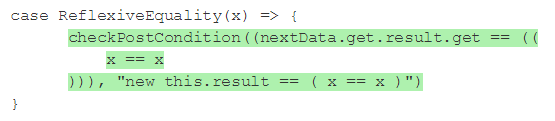
\includegraphics[width=\linewidth]{figures/eval_e0_reflexive-equality}
}
\caption{Test coverage example for \textit{ReflexiveEquality}}
\label{fig:ch3_eval_e0_highlighting_reflexive-equality}
\centering
\end{figure}
\FloatBarrier
% End figure
\pinfo{Property coverage}
The logic of a specification is defined in one Class in the generated system, which is called \textit{Logic} and prefixed by the specification name. We will only look at these classes to check to which extent the properties have been tested, using the highlighting that shows the coverage.\\
\\
\pinfo{Won't reach 100\%}
The generated system also contains some other logic that is more related to how it communicates with other instances when it is deployed, which is not something that we test. As a result, we will not be able to bring the test coverage to 100\%. However, all files in the generated system will be used to determine the overall coverage percentage. Since we use the same SUT to determine the coverage of the test suite on the SUT, the higher the coverage, the more complete it tests the defined properties in the generated system.

% Amount of bugs
\subsubsection{Amount of bugs}
\pinfo{Not a hard criteria, still using for indication}
The number of bugs found by an experiment also describes how effective the experiment was. Although this can not be a hard criteria, as it can vary per case. Consider that the system was already tested thoroughly, such that the bugs that this test suite would have found are already solved. This would mean that the amount of bugs found would remain 0, thus wouldn't have any effect as criteria. It is still an interesting part, as the amount of bugs found proofs that the test suite is able to find bugs. Because of this, we will report on this criteria and take it into account, but it will not be a critical criteria on determining whether one experiment was more successful than the other.

%\todo[inline]{Efficiency? Not yet.\\
%Can be done like getting coverage of libraries too, then substitute amount of properties and show that the same coverage can be received with less property tests. Thus less test cases, faster speed, same coverage. However, this would entail that the amount of bugs could go lower, as certain specific properties wont be tested if we require only coverage.}


% % % % % % % % % % % % % % % % % % % % % % % % % % % % % % % % % % % % %
% Section: Conclusion
\section{Conclusion}
\pinfo{Our approach, like QuickCheck}
The research question for this chapter lead as follows:\rqTwo{}. Existing approaches often require the SUT to be written in the same language. This was not possible when testing the generator in our case. The generator is being used to generate a system that is being used to test the generator. We use an approach that is similar to QuickCheck but using a \textit{Rebel} specification and the generated system to check whether the properties hold when using the generator.\\
\\
\pinfo{Combining all steps}
We demonstrated a full cycle based on one property, which indicated that this approach works to check a property. A full cycle consists of the following 5 phases:
\begin{enumerate}
\item \tfPhaseOne{}
\item \tfPhaseTwo{}
\item \tfPhaseThree{}
\item \tfPhaseFour{}
\item \tfPhaseFive{}
\end{enumerate}
The first step is done manually by translating the properties to a consistent \textit{Rebel} specification. The test framework is able to execute the other phases, which can be found in the \code{Main.rsc} file in the source code of this project.\\
\\
\pinfo{Larger specification for experiments}
For the experiments all the properties defined in \autoref{cpt:properties} will be used. This results in a bigger specification which can be used to test the generator automatically by using the test framework. After running the test framework, we evaluate it on the coverage and amount of bugs found metrics. The event definitions of each property defined in \autoref{cpt:properties} can be found in \autoref{app:a_event_definitions}.

% % % % % % % % % % % % % % % % % % % % % % % % % % % % % % % % % % % % %
% Section: Threats to validity
\section{Threats to validity}

\subsection*{Uncompilable system}
When the SUT is unable to compile, the test framework cannot proceed. As it cannot run the generated test suite against the SUT in that case. Although such errors could be detected by the test framework, it is out of scope for this thesis. IT is hard to argue whether the compilation error would be a bug or something else, as it can have many causes. However, when running the test framework this might still occur, which is a threat to this approach.

\subsection*{Accuracy}
\pinfo{Possibly incorrect results, due to Scoverage}
To evaluate the test framework we use coverage as a metric, which could have reported incorrect results. Scoverage is being used to determine the coverage and to generate a report from it. Since we are using random data as input, the results of the test coverage can fluctuate by small amounts in each run. However, we can still reason about the differences when there is a big difference between certain experiments. Additionally to the coverage we used the number of bugs that were found as another metric. This metric depends on which system the test suite is being run and if the system already fixed the bugs that the test suite would find. It is also the case that after fixing the bugs that were found earlier, this metric can be seen as unnecessary, as it would result in 0 then.

\subsection*{One system}
\pinfo{Only one generator}
Only one generator is being used throughout this thesis. However, it could be useful to make the test framework compatible with the other generators and generated systems too. This enables reasoning about the different implementations and its generators. Some changes are required to make the test framework compatible with these systems. But by doing so, every generated system for which a generator is built by ING can be checked based on the same properties, resulting in that the defined properties are checked thoroughly on every system and that inequalities can be detected between the different generators.\\
\\
\pinfo{Probably causing compile errors}
A threat in doing so is that one of the other generators might not support some translations of each expression that is used in the specification that we created. Thus this test framework can also be used to check whether every expression variant is taken into account by the generator. Unfortunately, an error in this translation would be blocking, in that it can lead to a generated system that is not able to compile. Resulting in that the test framework cannot proceed to run the test suite on the generated system. This could be used as a way to check the generators too. Although compilation errors were not the aim of the project, as compilation errors can have many causes, the test framework can still be used to detect those to a certain extent.

\subsection*{Whitebox implementation}
\pinfo{ScalaCheck, not testing generator then}
We chose to use property-based testing and implement the required functionality ourselfes, resulting in a white-box implementation. This means that we expect that our values generation is working correctly too. In case this isn't working correctly, this has to be fixed too.\\
\\
Another way how this could be done was to check how the custom types were generated to \textit{Scala}. And then generate a \textit{Scala} test project using the same types. Writing property tests for each type could achieve the same goal when it comes to checking the implementation of this component in the generated system. However, if we would follow this approach, we wouldn't use the generator to translate the \textit{Rebel} expressions to \textit{Scala}. This results in that the generator itself is still not being tested. With our approach, we test the generator and are able to find errors in the generator. Although we cannot conclude that the generator is implemented correctly if the generated test suit runs successful, rather we can conclude that the properties it checks for are satisfied.

% % % % % % % % % % % % % % % % % % % % % % % % % % % % % % % % % % % % %
% Chapter: Experiment 1
% % % % % % % % % % % % % % % % % % % % % % % % % % % % % % % % % % % % %
\chapter{Experiment 1: Using random input}
\label{cpt:experiment1}
\pinfo{Props to test cases, implication returns True}
The properties that we defined in \autoref{cpt:4_properties} are translated into
test cases as described in \autoref{cpt:3_testmechanics}. In this experiment we
expect to find some bugs that were unknown before by using the test framework.
When we have triggered some bugs, an investigation is needed to check what the
cause is of that bug. Next, we can categorize the bugs found to come to an
answer to this research question:\rqThree{}

% % % % % % % % % % % % % % % % % % % % % % % % % % % % % % % % % % % % %
% Section: Method
\section{Method}
%\label{sec:initial_case}
\pinfo{Like QuickCheck, recall cycle shortly}
In the first experiment each property will be tested 100 times by random input
values. This means that if the property holds for 100 tests, it is reported to be successfully satisfying the property. This is a similar approach as what \textit{QuickCheck} does when
checking properties. Unlike \textit{QuickCheck}, the test framework does not shrink the input values to come with minimum values for which the case fails. Instead it will just report the values that were used when the property failed.

% % % % % % % % % % % % % % % % % % % % % % % % % % % % % % % % % % % % %
% Section: Results
\section{Results}
In this experiment two runs are being done to detect bugs in the generator. The
first run terminated quickly, which is why the test framework did not succeed in
testing every property.

% % % % % % % % % % % % %
% Subsection: First run
\subsection{First run}
\pinfo{Termination, compile error due to library}
The first run results into a termination of the run due to a compile error in the generated system. Although we made the assumption that the generated system should be compilable, this error came from a property definition that was expected to fulfill, namely \textit{AssociativeMultiplicationInteger1} (\autoref{ssct:4_associativity}). Which is why we can consider this as an error that is found when using the test framework. The error describes that an overloaded method cannot be applied to the \textit{Money} type, as shown in \autoref{lst:ch5_firstrun_termination_log}.
% Listing
\FloatBarrier
\begin{sourcecode}[h!]
\begin{lstlisting}[language=Log]
[error] MoneySpec.scala:316: overloaded method value * with alternatives:
[error]   (x: Double)Double <and>
[error]   (x: Float)Float <and>
[error]   (x: Long)Long <and>
[error]   (x: Int)Int <and>
[error]   (x: Char)Int <and>
[error]   (x: Short)Int <and>
[error]   (x: Byte)Int
[error]  cannot be applied to (squants.market.Money)
[error]           Initialised(Data(result = Some(((((x * y)) * z) == (x * ((y * z)))))))
[error]                                                                 ^
[error] MoneySpec.scala:441: overloaded method value * with alternatives:
[error]   (x: Double)Double <and>
[error]   (x: Float)Float <and>
[error]   (x: Long)Long <and>
[error]   (x: Int)Int <and>
[error]   (x: Char)Int <and>
[error]   (x: Short)Int <and>
[error]   (x: Byte)Int
[error]  cannot be applied to (squants.market.Money)
[error]             checkPostCondition((nextData.get.result.get == (((((x * y)) * z) == (x * ((y * z)))))), "new this.result == ( (x*y)*z == x*(y*z) )")
[error]                                                                                    ^
[error] two errors found
[error] (compile:compileIncremental) Compilation failed
[error] Total time: 79 s, completed 4-aug-2017 13:03:45
> Done testing
> ** Some tests failed! **
\end{lstlisting}
\caption{Log output first test run resulting in a termination.}
\label{lst:ch5_firstrun_termination_log}
\end{sourcecode}
\todo{Up arrow is incorrectly aligned in the listing due to layout}
\FloatBarrier
% End listing
\pinfo{Investigation, found property and var types}
The error log does not clearly indicate what is exactly going wrong, it also does not describe what the types of the variables were. Investigating the generated system reveals that both errors were happening when dealing with the \textit{AssociativeMultiplicationInteger1} property. This means that the variables x, y and z are of type \textit{Integer}, \textit{Integer}, \textit{Money} respectively, as described in \autoref{ssct:4_associativity}. Temporarily disabling this property allows the test framework to

% % % % % % % % % % % % %
% Subsection: Second run
\subsection{Second run}
\pinfo{Failing tests, describing each}
After disabling the \textit{AssociativeMultiplicationInteger1} property, the test framework was able to run completely. This results in 7 failing tests. For each test the input values for which the property doesn't hold are logged such that the error can be reproduced. In \autoref{tbl:experiment1_overview_second_run} an overview of the failing properties, along with it's input values are shown.
% Table
\FloatBarrier
\begin{table}[!ht]
\centering
\begin{tabular}{llll}
\hline
\textbf{Property name}               & \textbf{X}               & \textbf{Y}        & \textbf{Z}         \\ \hline
DistributivePercentage1              & 0.51                     & -311254801.77 EUR & -707194075.77 EUR  \\
DistributivePercentage2              & 0.93                     & 2089630160.75 EUR & -1316628389.49 EUR \\
DistributiveInt2                     & -883022216               & -298435082.93 EUR & 715725888.96 EUR   \\
AssociativeMultiplicationPercentage2 & 840296462                & 1771903729.60 EUR & 0.53               \\
AssociativeMultiplicationInteger2    & -1852801029.34 EUR       & -1309504561       & 1880170895         \\
DistributiveInt1                     & -1790274467.41 EUR       & 1691684272        & 1449321647         \\
AssociativeMultiplicationPercentage1 & -352883323.42 EUR        & 0.27              & 294211708          \\ \hline
\end{tabular}
\caption{Overview of failing tests along with its input values}
\label{tbl:experiment1_overview_second_run}
\end{table}
\FloatBarrier
% End table


% % % % % % % % % % % % % % % % % % % % % % % % % % % % % % % % % % % % %
% Section: Analysis
\section{Analysis}
For each failed test we investigate what went wrong. The first four tests reveal precision problems when using the \textit{Money} type in calculations. The latter three tests were initially also failing because of these precision problems. However, these tests were also failing after the precision errors were fixed. For the latter 3 tests another version of the generated system was used, which contains the fixes for the precision problems. This is done such that we are able to reveal the other errors that these properties can reveal.

\todo{Add red and bold in tables}
% % %
% Explaining failing cases.
% % %
% % %
% DistributivePercentage1
\subsubsection{DistributivePercentage1}
\label{ssct:ch5_distributivePercentage1}
This property uses a \textit{Percentage} value and two \textit{Money} values for it's tests. The values are named x, y and z respectively. To check this failing test, we check the results of the intermediate calculations in the formula that is being used. In \autoref{ch4_init_check_DistributivePercentage1} values are shown for which the test case fails, among with the intermediate calculations. The intermediate calculations seem to work as expected, as the results are the same when we compare the results of the Scala evaluation and the Rascal evaluation. Unfortunately the resulting left hand side of the expression contains a precision error, which is caused when multiplying a \textit{Percentage} (the x variable) with a \textit{Money} type (the result of y+z in this case).
% Table
\FloatBarrier
\begin{table}[!ht]
\centering
\begin{tabular}{rll}
\hline
\textbf{Variable}      & \textbf{Value}          & \textbf{Type}            \\ \hline
X                      & 0.51                    & Percentage               \\
Y                      & -311254801.77 EUR       & Money                    \\
Z                      & -707194075.77 EUR       & Money                    \\ \hline
\textbf{Formula}       & \textbf{Scala result}   & \textbf{Expected result} \\ \hline
x*(y+z) == (y*x)+(z*x) & false                   & true                     \\
x*(y+z)                & -519408927.54539996 EUR & -519408927.5454 EUR      \\
(y*x)+(z*x)            & -519408927.5454 EUR     & -519408927.5454 EUR      \\
                       &                         &                          \\
y+z                    & -1018448877.54 EUR      & -1018448877.54 EUR       \\
y*x                    & -158739948.9027 EUR     & -158739948.9027 EUR      \\
z*x                    & -360668978.6427 EUR     & -360668978.6427 EUR      \\ \hline
\end{tabular}
\caption{DistributivePercentage1: Precision error when multiplying a \textit{Percentage} with \textit{Money}}
\label{ch4_init_check_DistributivePercentage1}
\end{table}
\FloatBarrier
% End table

% % %
% DistributivePercentage2
\subsubsection{DistributivePercentage2}
This test case looks similar than the \textit{DistributivePercentage1} (\autoref{ssct:ch5_distributivePercentage1}). It uses the same type of variables, but the expression is slightly different. In \autoref{ch4_init_check_DistributivePercentage2} the result and the intermediate calculations of a failing case are shown. What can be seen here is that the precision error occurs when the Money type is multiplied by the Percentage type. While in \autoref{ssct:ch5_distributivePercentage1} it was the other way around.
% Table
\FloatBarrier
\begin{table}[!ht]
\centering
\begin{tabular}{rll}
\hline
\textbf{Variable}      & \textbf{Value}          & \textbf{Type}            \\ \hline
X                      & 0.93                    & Percentage               \\
Y                      & 2089630160.75 EUR       & Money                    \\
Z                      & -1316628389.49 EUR      & Money                    \\ \hline
\textbf{Formula}       & \textbf{Scala result}   & \textbf{Expected result} \\ \hline
(y+z)*x == (y*x)+(z*x) & false                   & true                     \\
(y+z)*x                & 718891647.2718 EUR      & 718891647.2718 EUR       \\
(y*x)+(z*x)            & 718891647.2718001 EUR   & 718891647.2718 EUR       \\
                       &                         &                          \\
y+z                    & 773001771.26 EUR        & 773001771.26 EUR         \\
y*x                    & 1943356049.4975002 EUR  & 1943356049.4975 EUR      \\
z*x                    & -1224464402.2257001 EUR & -1224464402.2257 EUR     \\ \hline
\end{tabular}
\caption{DistributivePercentage1: Precision error when multiplying a \textit{Money} with \textit{Percentage}}
\label{ch4_init_check_DistributivePercentage2}
\end{table}
\FloatBarrier
% End table

% % %
% DistributiveInt2
\subsubsection{DistributiveInt2}
\label{ssct:ch5_distributiveInt2}
This case uses \textit{Integer} in conjunction with the \textit{Money} type. Earlier cases showed that there was a precision error when using the \textit{Percentage} and \textit{Money} types. Since the \textit{Percentage} type is translated to a \textit{Double} in the generated system, it can be expected that there would be precision problems occuring. As this is a known issue with types that use floating-point arithmetic \cite{goldberg1991every}. This case reveals that a precision error also occurs when multiplying \textit{Money} with an \textit{Integer}. In the intermediate calculations when investigating a failing test with it's values are shown in \autoref{ch4_init_check_DistributiveInt2}. The last two rows, colored in red, show that a precision error occurs when \textit{Money} is multiplied by an \textit{Integer}.
% Table
\FloatBarrier
\begin{table}[!ht]
\centering
\begin{tabular}{rll}
\hline
\textbf{Variable}  & \textbf{Value}          & \textbf{Type}              \\ \hline
X                  & -883022216              & Integer                    \\
Y                  & -298435082.93 EUR       & Money                      \\
Z                  & 715725888.96 EUR        & Money                      \\ \hline
\textbf{Formula}   & \textbf{Scala result}   & \textbf{Expected result}   \\ \hline
(x*y)*z == x*(y*z) & false                   & true                       \\
(x*y)*z            & -368477052257036740 EUR & -368477052257036762.48 EUR \\
x*(y*z)            & -368477052257036796 EUR & -368477052257036762.48 EUR \\
                   &                         &                            \\
y+z                & 417290806.03 EUR        & 417290806.03 EUR           \\
y*x                & 263524808260992384 EUR  & 263524808260992372.88 EUR  \\
z*x                & -632001860518029180 EUR & -632001860518029135.36 EUR \\ \hline
\end{tabular}
\caption{DistributiveInt2: Precision error when multiplying Money with an Integer}
\label{ch4_init_check_DistributiveInt2}
\end{table}
\FloatBarrier
% End table

% % %
% AssociativeMultiplicationPercentage2
\subsubsection{AssociativeMultiplicationPercentage2}
The earlier cases already shown a precision error when using Doubles and Integers in conjunction with \textit{Money}. This case triggers the same problem, but also reveals that the same thing happens when multiplying an \textit{Integer} with \textit{Money}. While in \autoref{ssct:ch5_distributiveInt2} it was the other way around. The intermediate calculations are shown in \autoref{ch4_init_check_AssociativeMultiplicationPercentage2}, the calculation of multiplying an Integer with Money is shown in red. Additionally, this case shows that the small precision error that we've seen earlier can cause a seemingly difference, which is a difference of 130 EUR in this case.
% Table
\FloatBarrier
\begin{table}[!ht]
\centering
\begin{tabular}{rll}
\hline
\textbf{Variable}  & \textbf{Value}          & \textbf{Type}              \\ \hline
X                  & 840296462               & Integer                    \\
Y                  & 1771903729.60 EUR       & Money                      \\
Z                  & 0.53                    & Percentage                 \\ \hline
\textbf{Formula}   & \textbf{Scala result}   & \textbf{Expected result}   \\ \hline
(x*y)*z == x*(y*z) & false                   & true                       \\
(x*y)*z            & 789129950543366910 EUR  & 789129950543366877.856 EUR \\
x*(y*z)            & 789129950543366780 EUR  & 789129950543366877.856 EUR \\
                   &                         &                            \\
x*y                & 1488924434987484670 EUR & 1488924434987484675.2 EUR  \\
y*z                & 939108976.688 EUR       & 939108976.688 EUR          \\ \hline
\end{tabular}
\caption{AssociativeMultiplicationPercentage2: Precision error causing bigger differences}
\label{ch4_init_check_AssociativeMultiplicationPercentage2}
\end{table}
\FloatBarrier
% End table

% % %
% AssociativeMultiplicationInt2
\subsubsection{AssociativeMultiplicationInteger2}
% - Integer overflows, causing negative values etc.
For this case three variables are used: x, y and z, which are of type \textit{Money}, \textit{Integer} and \textit{Integer} respectively. In \autoref{ch4_init_check_AssociativeMultiplicationInteger2} the values of a failing test case are shown with the intermediate formula steps. On the left side of the expression we see the expected results, while on the right side there is a big difference. The red colored row shows a huge difference in the resulting values between Scala and the expected value of the intermediate step on this expression. The result value of the operation is smaller than the minimum value of an \textit{Integer}. Causing it to underflow, resulting in an unexpected amount as result. Thus the operation neither checks for underflowing an \textit{Integer} value, nor does it prevent it.\todo{SOURCE-Over/underflow}
% Table
\FloatBarrier
\begin{table}[!ht]
\centering
\begin{tabular}{rll}
\hline
\textbf{Variable}  & \textbf{Value}                      & \textbf{Type}                       \\ \hline
X                  & -1852801029.34 EUR                  & Money                               \\
Y                  & -1309504561                         & Integer                             \\
Z                  & 1880170895                          & Integer                             \\ \hline
\textbf{Formula}   & \textbf{Scala result}               & \textbf{Expected result}            \\ \hline
(x*y)*z == x*(y*z) & false                               & true                                \\
(x*y)*z            & 4561767263499657218201769467.30 EUR & 4561767263499657218201769467.30 EUR \\
x*(y*z)            & 3877739486117270379.94 EUR          & 4561767263499657218201769467.30 EUR \\
                   &                                     &                                     \\
x*y                & 2426251398546224819.74 EUR          & 2426251398546224819.74 EUR          \\
y*z                & -2092906591                         & -2462092362461952095                \\ \hline
\end{tabular}
\caption{AssociativeMultiplicationInteger2: \textit{Integer} underflows when using multiply}
\label{ch4_init_check_AssociativeMultiplicationInteger2}
\end{table}
\FloatBarrier
% End table

% % %
% DistributiveInt1
\subsubsection{DistributiveInt1}
This case also uses three variables: x, y and z. Which are of type \textit{Money}, \textit{Integer} and \textit{Integer} respectively. In \autoref{ch4_init_check_DistributiveInteger1} the different values are shown of the calculation between Scala and the expected result. The red line shows how the addition of two (positive) Integers results in a negative value. The result value would be bigger than the maximum value of an \textit{Integer}, causing it to overflow. Thus the operation also does not check or prevent against overflowing. \todo{SOURCE-Over/underflow}
% Table
\FloatBarrier
\begin{table}[!ht]
\centering
\begin{tabular}{rll}
\hline
\textbf{Variable}      & \textbf{Value}              & \textbf{Type}               \\ \hline
X                      & -1790274467.41 EUR          & Money                       \\
Y                      & 1691684272                  & Integer                     \\
Z                      & 1449321647                  & Integer                     \\ \hline
\textbf{Formula}       & \textbf{Scala result}       & \textbf{Expected result}    \\ \hline
x*(y+z) == (x*y)+(x*z) & false                       & true                        \\
x*(y+z)                & 2065907589620385223.57 EUR  & -5623262698769382599.79 EUR \\
(x*y)+(x*z)            & -5623262698769382599.79 EUR & -5623262698769382599.79 EUR \\
                       &                             &                             \\
y+z                    & -1153961377                 & 3141005919                  \\
x*y                    & -3028579159080673575.52 EUR & -3028579159080673575.52 EUR \\
x*z                    & -2594683539688709024.27 EUR & -2594683539688709024.27 EUR \\ \hline
\end{tabular}
\caption{DistributiveInteger1: \textit{Integer} overflows when using addition}
\label{ch4_init_check_DistributiveInt1}
\end{table}
\FloatBarrier
% End table

% % %
% AssociativeMultiplicationPercentage1
\subsubsection{AssociativeMultiplicationPercentage1}
% - Generating big double, precision can't be known for Squants!
In this case there are three variables: x, y and z, which are of type
\textit{Money}, \textit{Percentage} and \textit{Integer} respectively. In Table
\ref{ch4_init_check_AssociativeMultiplicationPercentage1} the values and
intermediate calculations are shown of a failing case, such that we can reason
about the results. The row marked in red shows a precision error when comparing
the results of Scala and Rascal with each other. This issue is caused by the
\textit{Percentage} that is being used. In the implementation, the
\textit{Percentage} is actually being translated into a \textit{Double}, which
is being multiplied with an \textit{Integer}. This results in a \textit{Double}
value containing a precision error, which is related to the problems with
floating-point arithmetic \cite{goldberg1991every}.
% Table
\FloatBarrier
\begin{table}[!ht]
\centering
\begin{tabular}{rll}
\hline
\textbf{Variable}  & \textbf{Value}         & \textbf{Type}               \\ \hline
X                  & -352883323.42 EUR      & Money                       \\
Y                  & 0.27                   & Percentage                  \\
Z                  & 294211708              & Integer                     \\ \hline
\textbf{Formula}   & Scala result           & Expected result             \\ \hline
(x*y)*z == x*(y*z) & false                  & true                        \\
(x*y)*z            & -28032049433190944 EUR & -28032049433190942.3672 EUR \\
x*(y*z)            & -28032049433190948 EUR & -28032049433190942.3672 EUR \\
                   &                        &                             \\
x*y                & -95278497.3234 EUR     & -95278497.3234 EUR          \\
y*z                & 79437161.16000001      & 79437161.16                 \\ \hline
\end{tabular}
\caption{AssociativeMultiplicationPercentage1: A precision error when using \textit{Percentage}}
\label{ch4_init_check_AssociativeMultiplicationPercentage1}
\end{table}
\FloatBarrier
% End table
Additionally, we can see a difference in the results on the left and right side of the expression evaluation in Scala. Where as the intermediate step for the left side is calculated correctly. This also hints to the bug in the \textit{Money} type which we already found with the `DistributiveInt2` test. For the right side we cannot say this immediately, as there is already an error in the intermediate step.\\
\\
This property revealed a precision error when the \textit{Percentage} type is being used. The \textit{Percentage} is being translated to a \textit{Double} value, causing operations with it to have precision errors. In this case the \textit{Percentage} is being multiplied by an \textit{Integer}.

% % % % % % % % % % % % % % % % % % % % % % % % % % % % % % % % % % % % %
% Section: Evaluation criteria
\section{Evaluation criteria}

% Property coverage
\pinfo{Not tested implicative properties}
When looking at the coverage results of the test suite, it is notable that the if-clause of the implicative properties are often not satisfied. As shown in Figure X, green highlighting indicate the statements that are executed, while red highlighting indicate statements that were not checked at all. As a result, the property always returns \textit{true}, as this is how it was specified in the specification (the else-clause of an implicative property). This is due to the random values that are being used as input. An example of this is the Transitive property (\code{x == y \&\& y == z $\implies$ x == z}). When relying on random data, there is a seldom chance that 3 values are equal to each other. Thus we could optimize the random values such that the condition holds, such that we also test these properties such that the if-clause is triggered.\\
\\
\textbf{Figure X}
\todo{Add figure}

% Total coverage
\pinfo{Test coverage, 30\% for implicative, 100\% for others}
The first criteria to evaluate an experiment was to determine the test coverage. The properties using implication are not covered when using random values as input data. The other properties, which do not use implication, are fully tested though. This can be seen in Figure X, where the test coverage of the properties using implication only covers roughly 30\%. The files with a name ending with "Logic" contain the implementation of the properties, as well as the precondition checks. The test coverage concerning the other properties (those that do not use implication), reports 95\% coverage. When investigating further, the other 5\% are not related to the properties that we test, thus it is not required for this project to achieve 100\% coverage on the Logic files.\\
\begin{figure}[h!]
\frame{
	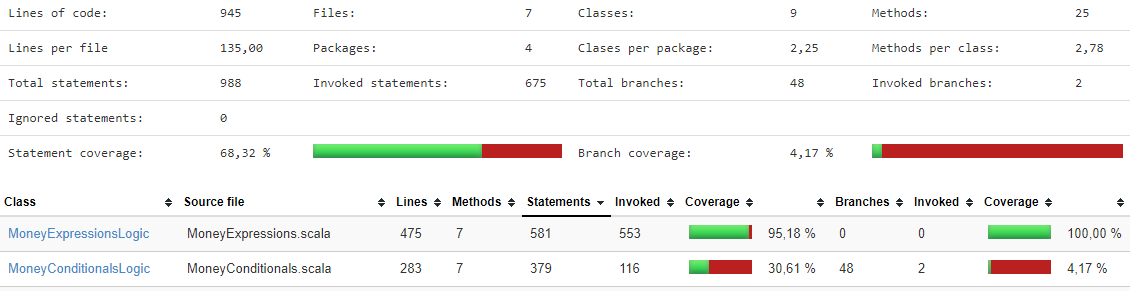
\includegraphics[width=\linewidth]{figures/eval_experiment1}
}
\caption{Test coverage report of the first experiment}
\label{fig:ch5_eval_experiment1}
\centering
\end{figure}
\\
\pinfo{Overall 68\%, cannot be 100, but can be improved}
The overall coverage over the generated system is 68\%, however, note that the generated system is based on the properties that we defined and that the libraries that are being used by the generated system are not included in the coverage report. The generated system also contains some other logic that is more related to how it communicates with other instances when it is deployed, which is not something that we test. As a result, we will not be able to bring the test coverage to 100\%. Although the test suite can be improved to have a higher test coverage, by generating values such that the properties using implication are also triggering the if-clause. Which is currently not the case, as we have seen when checking the coverage of each property in Figure X-1.\\
\\
% % of bugs
\pinfo{\# of bugs, 7}
The second criteria that we defined was the amount of bugs that we have found by doing the experiment. By using this approach we found a total of 4 bugs. A compilation error, overflow/underflow error and precision errors. 2 of these 4 bugs were related to the precision problem when using doubles, but one originated from the library that is used for the Money type, while the other is because the \textit{Percentage} type is translated to a \textit{Double}. Which is why we define these as 2 separate bugs. An improvement of the test suite to also cover the properties using implication might result in more bugs that can be found.

% % % % % % % % % % % % % % % % % % % % % % % % % % % % % % % % % % % % %
% Section: Conclusion
\section{Conclusion}
% 1: Squants using doubles internally. Small precision error can lead to bigger (unexpected) amounts as we've seen in AMP2.
% 	 - DistributivePercentage1: Multiplying Double with Money causes a precision error
%	 - DistributivePercentage2: Multiplying Money with Double causes a precision error
% 	 - DistributiveInt2: Multiplying Money with Integer
%    - AssociativeMultiplicationPercentage2: Multiplying Integer with Money. And with double. Causing big numbers to be losing precision anyway. Bug in Squants is the problem here though.
% 2: Operations on an Integer are over/underflowing, causing incorrect results.
%	 - AssociativeMultiplicationInt2: When using Multiply on Ints
%	 - DistributiveInt1: When using Addition on Ints
% 3: Percentage is double, causing big values to lose precision, which can cascade through the expressions
%	 - AssociativeMultiplicationPercentage1: Multiplying Percentage with Int, causing a big Double value with precision loss. Squants cannot guess the actual number anymore
\pinfo{Recap, found 7 bugs using this approach}
In this first experiment we tested each property that was defined in \autoref{cpt:4_properties} 100 times with using random values as input. First the test suit terminated due to a compilation error. After disabling the causing property (temporarily), a total of 7 tests were failing. In this experiment we managed to find precision errors and overflow/underflow errors. Additionally, we found a compilation error when using a property which was expected to hold.

% % % % % % % % % % % % % % % % % % % % % % % % % % % % % % % % % % % % %
% Section: Threats to validity
\section{Threats to validity}

\subsection*{Fixed amount of tries}
\pinfo{Fixed amount of tries not substantiated}
The 100 tries to check a property is a fixed number that is being used. But why exactly this number and not a higher or lower number? It might be the case that some errors are not triggered because of this fixed amount. Running more cases might be revealing an additional error, or it might not. In case it doesn't, it means that the test suite just requires more time to run the whole test suite, while it does not have an effect on the results. 100 seems to be an amount that works such that it consistently reports the same amount of failing tests, however this has checked by running it the test runs multiple times, also with using numbers like 300 or 50 for the amount. Also \textit{QuickCheck} uses this amount to check a property. During this thesis we stick with 100 as amount. Finding the optimal amount of tries is left as future work, thus remaining as a threat of validity in this approach.

\subsection*{Unfixed issue}
\pinfo{Compile error not fixed}
Unfortunately the compilation error has not been fixed throughout this project, however, it is an open issue on \textit{Github}. Some precision errors originated from a library used in the generated system, called Squants. An issue was created covering these precision errors, which were fixed in the next release of that library. As for the overflow and underflow errors, these occurred when using the \textit{Integer} type in \textit{Rebel}. When using the \textit{Integer} type, this might have been expected behaviour which causes this to happen. However, the generated system does not check whether this happens, nor does it prevent this. Additionally, we can consider this behaviour unexpected on the Integer type in
\textit{Rebel}, as \textit{Rebel} does not support any other kind of number type that can hold a bigger value. For example, compared to
Java, a \textit{BigDecimal} would be possible. We consider the overflow and underflow errors as unexpected, as the \textit{Rebel} language does not support other numeric types to hold a bigger value than an \textit{Integer} supports.

% % % % % % % % % % % % % % % % % % % % % % % % % % % % % % % % % % % % %
% Chapter: Experiment 2
% % % % % % % % % % % % % % % % % % % % % % % % % % % % % % % % % % % % %
\chapter{Experiment 2: Smarter values generation}
\label{cpt:experiment2}
% % % % % % % % % % % % % % % % % % % % % % % % % % % % % % % % % % % % %
% Section: Smarter values generation
%\section{Smarter values generation}
%\label{sec:ch4_smarter_values_generation}
\pinfo{Context - result of experiment 1, what aim is now}
Some bugs were found by using random input values in the first experiment.
However, the implicative properties were not effectively checked in terms of
triggering the if-clause when using random input values. This is what we aim to
improve in this experiment, expecting to detect more bugs.

% % % % % % % % % % % % % % % % % % % % % % % % % % % % % % % % % % % % %
% Section: Method
\section{Method}
\label{sct:experiment2_method}
\pinfo{2 categories separation}
We can separate the properties that we have in 2 different categories: those
using implication ($\implies$) and those that do not. The defined properties are
being separated over two specifications according to which category these
belong. We name these specifications \textit{MoneyExpressions} and
\textit{MoneyConditionals}. For the \textit{MoneyConditionals} specification
(the implicative properties), another way of generating the random values is
more useful. The random input values are being optimized such that the condition
of the if-clause of these properties are being satisfied. For the other
specification (\textit{MoneyExpressions}), the earlier approach (random values
as input) can still be used. We do not need to change this functionality for
these cases since the properties can be used with random values.\\
\\
\pinfo{Adding preconditions}
In the \textit{MoneyConditionals} specification, the condition to trigger the
if-clauses will be added to the preconditions of each the event definition, such
that these can be used to generate the values matching this clause. The updated
event definition of the \textit{Symmetric} property is shown in
\autoref{lst:experiment2_updated_definition} for example. Where the
preconditions have been added to the event definition.
% Listing
\begin{sourcecode}[!ht]
\begin{lstlisting}[language=Rebel]
event symmetric(x: Money, y:Money) {
    preconditions {
        x == y;
    }
    postconditions {
       new this.result == ( (x == y) ? y == x : False );
    }
}
\end{lstlisting}
\caption{The updated event definition of the \textit{Symmetric} property}
\label{lst:experiment2_updated_definition}
\end{sourcecode}
\FloatBarrier
% End listing
\pinfo{Generating checks for preconditions}
When generating the test suite, the events are being traversed. In case an
event with some preconditions is found, it generates a list of value tuples that
satisfy the condition to trigger the if-clause. Which is different compared to
the generated tests in \autoref{cpt:experiment1}. The size of the tuples depends
on the arity of the event from which the test is being generated.\\
\\
\pinfo{Diff1: custom generator}
The first difference is that it now uses our custom generator to determine the
input values, instead of the built-in Java random generator. A list of tuples,
containing values which satisfy the if-clause of the implication, is being
generated. Our custom generator is a simple proof of concept in order to check
if this will actually result in more failing tests. This custom generator
basically consists of multiple methods which are being called based on the event
name. In \autoref{lst:ch4_second_generating_values} this behaviour is shown for
the \textit{Symmetric} and \textit{Division1} event. The \textit{String}
parameter of these methods is a way how we can pattern match on the event name
in \textit{Rascal}. In case the event couldn't be handled, an exception is
thrown.
% Listing
\begin{sourcecode}[!ht]
\begin{lstlisting}[language=Rascal]
private list[Expr] genTestValueForEvent("Symmetric") {
    Expr moneyValue = genRandomMoney();
    return [moneyValue, moneyValue];
}
private list[Expr] genTestValueForEvent("Division1") {
    real moneyAmountX = genRandomDouble();
    real intAmountY = genRandomInteger();
    real moneyAmountZ = moneyAmountX * intAmountY;
    str currency = genRandomCurrency();
    return [convertToMoney(currency, moneyAmountX), converToExpr(intAmountY), convertToMoney(currency, moneyAmountZ)];
}
private default list[Expr] genTestValueForEvent(str eventName) {
    throw "genTestValueForEvent not implemented for event <eventName>";
}
\end{lstlisting}
\caption{Values generation for \textit{Symmetric} and \textit{Division1}, including the fall-back case.}
\label{lst:ch4_second_generating_values}
\end{sourcecode}
\FloatBarrier
% End listing
\pinfo{Not very dynamic}
This means that the way how we determine these values is basically hard-coded,
requiring to have knowledge about the if-clause itself. Note that this doesn't
make this approach very dynamic, but the result will consist of a list of tuples
that satisfy the if-clause. These tuples will be used as input for the test case
that will be generated.\\
\\
\pinfo{Mutating values with random operation}
However, the values that are generated now are fixed when we use them directly
in a test case, which completely removes the randomness of the values when
running the tests. It would be better to keep the randomness, such that the
values are different on each run. To solve this problem, we mutate the values in
the list such that the values are sort of random again. The tuples still have to
satisfy the condition to trigger the if-clause, as this was the actual
intention. So the second difference compared to the first experiment, is that
for each tuple in the list, we will generate a random operation and use that
operation to mutate the values inside the tuple. To ensure that the tuple values
still satisfy the condition of the if-clause, each value in the tuple will be
mutated by the same operation. In
\autoref{lst:experiment2_second_resulting_test} an example of a generated test
case is shown.
% Listing
\begin{sourcecode}[!ht]
\begin{lstlisting}[language=Scala]
"work with Antisymmetry" in {
      Seq((USD(1593.62), USD(1593.62)), (USD(2869.78), USD(2869.78)),
          (EUR(4676.80), EUR(4676.80)), (USD(1850.29), USD(1850.29)),
          // ... // More values in the list
          (USD(9501.16), USD(9501.16)), (- EUR(149.67), - EUR(149.67)),
          (- EUR(159.67), - EUR(159.67)), (EUR(8015.77), EUR(8015.77)))
      .foreach {
        data:  (Money, Money) => {
          val randomOperation = genRandomOperation(genRandomOperator("Money", true), generateRandomMoney(data._1.currency), generateRandomInteger(true), generateRandomInteger(false), generateRandomPercentage(true), generateRandomPercentage(false), Random.nextInt(10))

          checkAction(Symmetry(
              randomOperation(data._1),
              randomOperation(data._2)
              )
          )
        }
      }
    }
\end{lstlisting}
\caption{Resulting test case with semi-random values. Omitted some input tuples for readability.}
\label{lst:experiment2_second_resulting_test}
\end{sourcecode}
\FloatBarrier
% End listing
\pinfo{Small explanation about the new test case}
The list of values are generated by using our custom generator, the number of
tuples in the list can be defined when generating the test suit. A method
\code{genRandomOperation()} has been added to the template, which is used to
mutate the fixed values in the list. After all the \code{checkAction()} method
is being called to check the result of the test.\\
\\
\pinfo{Also: else now returns false}
Now that the input values for the implication events should always satisfy the
condition of the if-clause, we can also update the specification such that the
else-clause of the expression always returns \textit{False}. This can be seen in
\autoref{lst:experiment2_updated_definition}. This results in a failing case
again in case the precondition was not met. When this happens, it could indicate
that there's a problem with either our custom generator or in the generator.

% % % % % % % % % % % % % % % % % % % % % % % % % % % % % % % % % % % % %
% Section: Results
\section{Results}
\pinfo{Failing tests: Division}
Running the test framework with these changes results in 2 additional failing tests
compared to the first experiment (\autoref{cpt:experiment1}). An overview of the
failing properties and the used input values are shown in
\autoref{tbl:experiment2_overview_first_run}. The log of the test run reports
that the precondition was not met when using these input values, as shown in
\autoref{lst:experiment2_log_first_run}.
% Table
\begin{table}[!ht]
\centering
\begin{tabular}{llll}
\hline
\textbf{Property name} & \textbf{x}    & \textbf{y} & \textbf{z} \\ \hline
Division1              & -16729.90 USD & 830        & -20.16     \\
Division2              & -44.68 USD    & 870        & -38870.47  \\ \hline
\end{tabular}
\caption{Failing tests overview along with its input values}
\label{tbl:experiment2_overview_first_run}
\end{table}
\FloatBarrier
% End table

% Listing
\begin{sourcecode}[!ht]
\begin{lstlisting}[language=Log]
[info] MoneyConditionals
[info] - should work with Additive4params (7 seconds, 224 milliseconds)
[info] - should work with AntisymmetryLET (5 seconds, 493 milliseconds)
[info] - should work with Symmetric (5 seconds, 344 milliseconds)
[info] - should work with Division2 *** FAILED *** (23 milliseconds)
[info]   java.lang.AssertionError: assertion failed: expected CommandSuccess(Division2(-16729.90 USD,830,-20.16 USD)), found CommandFailed(NonEmptyList(PreConditionFailed(x == z*y)))
[info] - should work with Division1 *** FAILED *** (127 milliseconds)
[info]   java.lang.AssertionError: assertion failed: expected CommandSuccess(Division1(-44.68 USD,870,-38870.47 USD)), found CommandFailed(NonEmptyList(PreConditionFailed(x*y == z)))
// ...
\end{lstlisting}
\caption{Precondition failed error in \textit{Division1} and \textit{Division2}.}
\label{lst:experiment2_log_first_run}
\end{sourcecode}
\FloatBarrier
% End listing

% % % % % % % % % % % % % % % % % % % % % % % % % % % % % % % % % % % % %
% Section: Analysis
\section{Analysis}
The values used in the test case should be correct since we generated these
values such that they satisfy the condition of the if-clause and thus they
should satisfy the preconditions. Note that the conditions of the if-clause were
added as preconditions in the \textit{MoneyConditionals} specification, which
causes the error. As the \textit{PreConditionFailed} error is thrown by the
system when the input values do not satisfy the preconditions.\\
\\
\pinfo{Describe precision error happening at first}
For \textit{Division1} it states that the condition \code{x*y == z} failed. The
values used for \textit{x}, \textit{y} and \textit{z} were \textit{-44.68 USD},
\textit{870} and \textit{-38870.47 USD} respectively. The result of
\textit{x * y} = \textit{-44.68 USD * 870} = \textit{-38871.60 USD}. This should
be equal to \textit{z}. In fact, the input of \textit{z} was slightly different,
\textit{-38870.47 USD}.\\
\\
Remember that the input values are being mutated by a random operation that we
have added to the test cases. This difference is caused by the precision error
when operating with the \textit{Money} type, which was found in
\autoref{cpt:experiment1}. The random operation that was done was causing this
behaviour. The same goes for the error with \textit{Division2}, where
\code{x == z*y} should hold. The values of \textit{x}, \textit{y} and \textit{z}
are \textit{-16729.90 USD}, \textit{830}, \textit{-20.16 USD} respectively. The
result of \textit{z * y} = \textit{-16732.80 USD}, which is not equal to
\textit{-16729.90} USD.\\
\\
\pinfo{Next (when fixed precision), division problem}
The first experiment already described the precision problem and how it could
be fixed. To solve this problem, we modify the generator such that the precision
error is fixed when generating the system. Then the test framework is being
executed again to check whether both tests are succeeding. This resulted in the
same amount of tests that were failing, which means that we found a different
case now. In \autoref{tbl:experiment2_overview_second_run} an overview of the
used input values are shown\footnote{The decimals have been truncated for
readability, \autoref{lst:experiment2_log_second_run} shows the exact values}.
The log reported that one case still fails on the precondition check, while the
other case just reports values for which the result is \textit{false}, as shown
in \autoref{lst:experiment2_log_second_run}.
% Table
\begin{table}[!ht]
\centering
\begin{tabular}{llll}
\hline
\textbf{Property name} & \textbf{x}                               & \textbf{y} & \textbf{z}                               \\ \hline
% Division1              & 1.504347826086956521739130434782609 USD  & -779       & -1171.886956521739130434782608695652 USD \\
Division1              & 1.5043478260... USD     & -779       & -1171.8869565217... USD \\
% Division2              & -3328.825454545454545454545454545455 USD & -129       & 25.80484848484848484848484848484848 USD  \\ \hline
Division2              & -3328.8254545454... USD & -129       & 25.8048484848... USD    \\ \hline
\end{tabular}
\caption{Failing tests overview, after fixing precision errors}
\label{tbl:experiment2_overview_second_run}
\end{table}
\FloatBarrier
% End table

% Listing
\begin{sourcecode}[!ht]
\begin{lstlisting}[language=Log]
[info] MoneyConditionalsSpec:
[info] MoneyConditionals
[info] - should work with Additive4params (7 seconds, 24 milliseconds)
[info] - should work with AntisymmetryLET (3 seconds, 66 milliseconds)
[info] - should work with Symmetric (4 seconds, 361 milliseconds)
[info] - should work with Division2 *** FAILED *** (670 milliseconds)
[info]   java.lang.AssertionError: assertion failed: expected CommandSuccess(Division2(-3328.825454545454545454545454545455 USD,-129,25.80484848484848484848484848484848 USD)), found CommandFailed(NonEmptyList(PreConditionFailed(x == z*y)))
[info] - should work with Division1 *** FAILED *** (316 milliseconds)
[info]   java.lang.AssertionError: assertion failed: expected CurrentState(Result,Initialised(Data(None,Some(true)))), found CurrentState(Result,Initialised(Data(None,Some(false)))): With command: Division1(1.504347826086956521739130434782609 USD,-779,-1171.886956521739130434782608695652 USD)
// ...
\end{lstlisting}
\caption{Precondition failed error in \textit{Division1} and \textit{Division2}.}
\label{lst:experiment2_log_second_run}
\end{sourcecode}
\FloatBarrier
% End listing
\pinfo{Division2 triggers division problem}
The test concerning \textit{Division2} shows that the precondition check fails.
If we look at the input values, it can be seen that the \textit{Money} values
are a fractional number. As it contains many decimals and it rounds up at the
end. When operating with this rounded value, the resulting value is also
slightly different. As the generated system is implemented such that the
preconditions are being checked first, the \textit{PreConditionFailed} exception
is thrown. This leads to the issue of the division problem in which a number
cannot be equally divided. When defining the properties in
\autoref{cpt:properties}, we did not take this into account. Instead, we defined
that it should contain the exact value, which cannot be done in this case. This
should be defined in order to determine whether this is expected or incorrect.\\
\\
\pinfo{Division1 triggers difference in rounding problem}
% Division1 is defined as \code{x*y == z $\implies$ x == z/y}.
When looking at \textit{Division1}, we see another case as the input values
passed the precondition checks. This indicates that the values satisfy the
condition to trigger the if-clause of the property. However, the result of the
if-clause returns \textit{false}, showing us that the property does not hold
when using these input values. Thus a case has been found for which the
\textit{Division1} property doesn't hold. The investigation of the intermediate
calculation steps are shown in
\autoref{tbl:experiment2_division1_rounding_difference}. Note that the
\textit{Division1} property is defined as \code{x*y == z $\implies$ x == z/y}.

% Table
\begin{table}[!ht]
\centering
\begin{tabular}{rll}
\hline
\textbf{Variable}  & \textbf{Value}                                    & \textbf{Type}                                        \\ \hline
X                  & 1.504347826086956521739130434782609 USD           & Money                                                \\
Y                  & -779                                              & Integer                                              \\
Z                  & -1171.886956521739130434782608695652 USD          & Money                                                \\ \hline
\textbf{Formula}   & \textbf{Scala result}                             & \textbf{Expected result}                             \\ \hline
x*y == z           & true                                              & false                                                \\
x == z/y           & false                                             & false                                                \\
                   &                                                   &                                                      \\
x*y                & -1171.886956521739130434782608695652 USD          & -1171.886956521739130434782608695652\textbf{411} USD \\
z/y                & 1.504347826086956521739130434782608 USD           & 1.504347826086956521739130434782608 USD              \\ \hline
\end{tabular}
\caption{Division1: Difference in rounding}
\label{tbl:experiment2_division1_rounding_difference}
\end{table}
\FloatBarrier
% End table
In the results, we can see that the expected values do not match the property
either. Although in \textit{Scala} the first expression is considered
\textit{true}. Since the expected results also return \textit{false} for the
intermediate calculations, the input values might not fully satisfy the
condition to trigger the if-clause. Which could be an implementation error in
our values generator. However, it's notable that in \textit{Scala} the condition
is considered to hold, which triggered this case. This indicates that there is a
rounding error happening in the system, which triggered this case.\\
\\
Unfortunately, we are unable to trace back how the input values used for this
tests were exactly determined. As these are build up by using randomly generated
values and then mutating these by a random operation (as described in
\autoref{sct:experiment2_method}). Nevertheless, the results show that there is
also an unexpected rounding going on when executing \textit{x*y} in
\textit{Scala}. As the expected value contains some additional decimals compared
to the result from \textit{Scala}.

% % % % % % % % % % % % % % % % % % % % % % % % % % % % % % % % % % % % %
% Section: Evaluation criteria
\section{Evaluation criteria}
\pinfo{Using 'fixed' version for evaluating}
To evaluate this experiment, we use the version of the generator in which the precision problems related to the \textit{Money} type are fixed. This is done because otherwise the precision errors would cause more tests to fail and the report would indicate a lower amount of coverage.\\
\\
\pinfo{Property coverage}
When looking at the coverage report concerning a specific implicative property,
it can be seen that the else-clause of the implication is not being triggered
anymore. This was also the intention of the modification done in this
experiment, as the if-clause is actually what we wanted to check in this
experiment. In
\autoref{fig:experiment2_eval_e2_highlighting_transitive-equality} the coverage
highlighting of \textit{TransitiveEquality} is shown.
% Figure
\begin{figure}[!ht]
%\frame{
	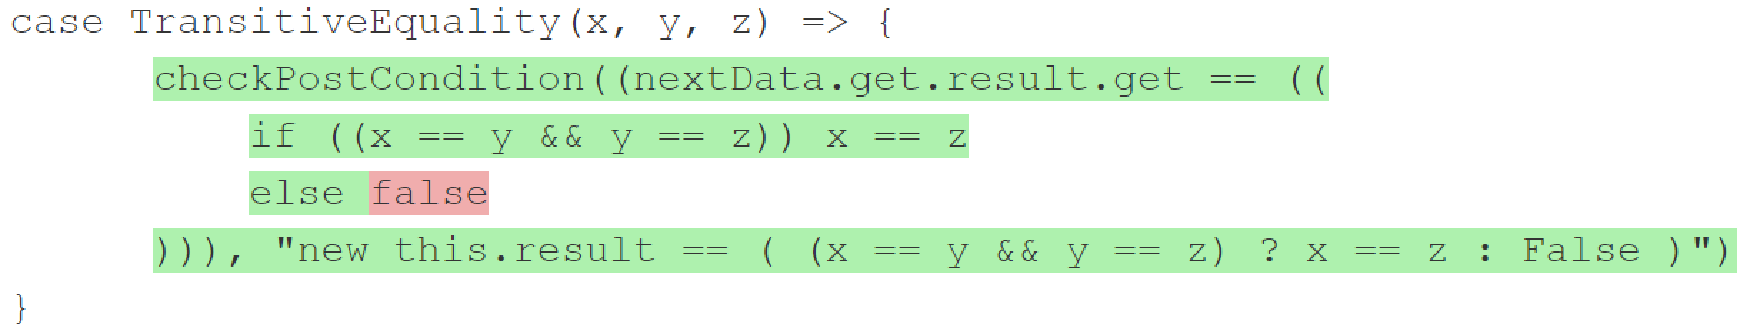
\includegraphics[width=\linewidth]{figures/e2_coverage_implicative_property}
%}
\caption{Test coverage for \textit{TransitiveEquality} in second experiment}
\label{fig:experiment2_eval_e2_highlighting_transitive-equality}
\centering
\end{figure}
\FloatBarrier
% End figure

% Evaluation criteria
\pinfo{88,87\% - image}
The expectation was that the test framework could be improved, such that the
test coverage on the generated system would become higher. In the first
experiment we found that the implicative properties were not tested thoroughly. This is what has been improved in this experiment. The coverage report does not indicate a huge difference compared to the first experiment (\autoref{cpt:experiment1}). The total test coverage is 88,87\%, which is slightly higher than the results in the first experiment. The report is shown in \autoref{fig:experiment2_eval_e2}. Note that the properties have been categorized in this experiment, this is also visible in the coverage report (the two ``Logic'' files, one for each category).
% Figure
\begin{figure}[!ht]
%\frame{
	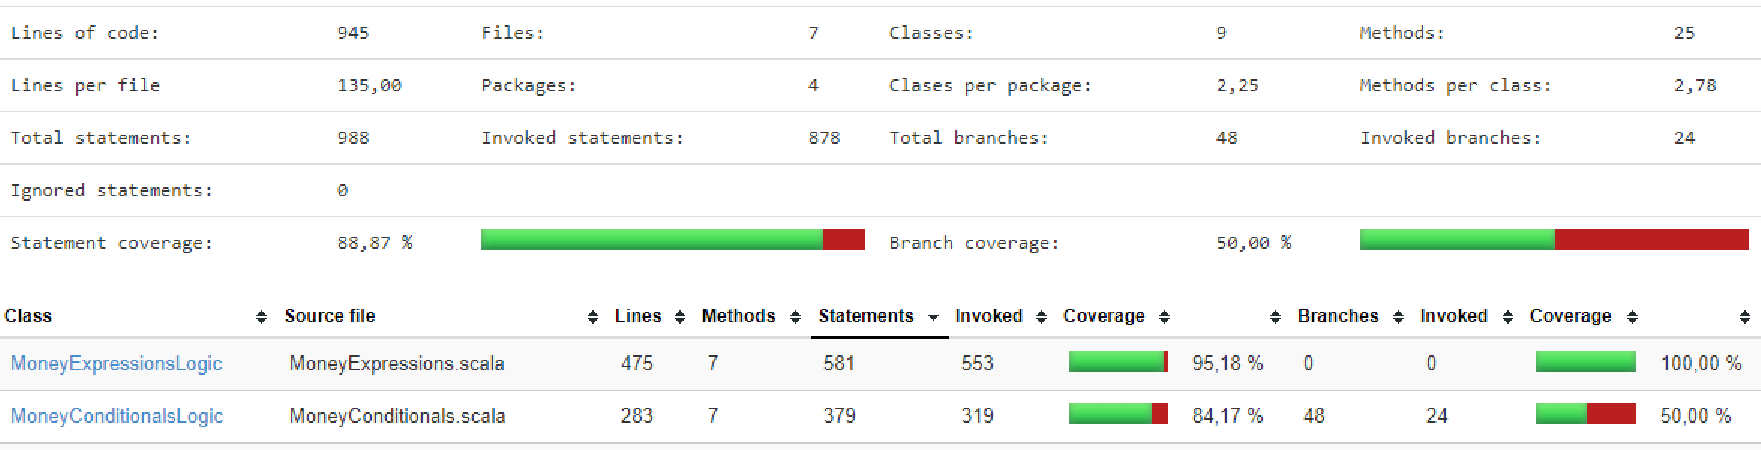
\includegraphics[width=\linewidth]{figures/eval_e2}
%}
\caption{Test coverage report of the second experiment}
\label{fig:experiment2_eval_e2}
\centering
\end{figure}
\FloatBarrier
% End figure
\pinfo{Branch coverage, 50\%}
It is notable from the coverage report that the branch coverage is exactly 50\%. This amount is lower than what it was in the first experiment. However, in this experiment the implicative properties are being tested thoroughly, which was not the case in the first experiment. Considering that the
else-clause of the implicative properties is not being triggered, the test
coverage will never become 100\%. Which is not a problem in that sense, as we
don't intend to test the else clause, we are more interested in the result of
the if-clause of these implicative properties. This is also true for the branch coverage, which can be expected to be 50\%. Although the first experiment reported a higher amount for this, it was not testing the implicative properties good enough in the first experiment.\\
\\
\pinfo{\# of bugs, 2 more, incorrect definition}
The other criteria we use was the number of bugs that we have found. Using this
approach 2 more tests were failing compared to the first experiment in
\autoref{cpt:experiment1}. The division problem was not taken into account when
defining the properties, which resulted in these failing cases.\\
\\
When defining the properties, it was stated that the value should be the exact
value, while this is not possible with division. This results in a threat to the
definition of this property. Because of this, we consider the bugs that were
found as false positives. Although, because of this it might be the case that
the actual bugs it might be able to find, are being hidden because of this.
Resulting in false negatives: bugs that exist in the system, but are not found
by the test framework.

% % % % % % % % % % % % % % % % % % % % % % % % % % % % % % % % % % % % %
% Section: Conclusion
\section{Conclusion}
In this experiment, we generated the input values such that the condition of
the implicative properties are satisfied. This revealed 2 additional
failing cases that are triggering the division problem. The generated system
tries to hold the exact value, which triggers this situation. It is reasonable
that the system tries to hold the exact value. It is also not clear from the
property definitions what should happen in this case.\\
\\
When defining the properties in \autoref{cpt:properties}, we said that a value
should be precise. However, it is not possible to do this for all division
cases. Because of this, we consider the bugs that were found as false positives.
The definition of the property has to be updated in order to specify what should
happen in case such a division error occurs. Due to this error, it might be the
case that existing bugs in the generator are not being detected with this
approach.\\
\\
The property definitions should be updated such that it is known what should
happen in this case. In the next experiment we will focus on improving this.

% % % % % % % % % % % % % % % % % % % % % % % % % % % % % % % % % % % % %
% Section: Threats to validity
\section{Threats to validity}

% Incorrect value generation
\subsection*{Incorrect value generation}
We have implemented a custom value generator to generate values for each test
case. Furthermore, a random operation is being done on these values to make
these random again. There could be an error in the implementation that incorrect
values are being created, which are expected to be correct values. When this is
the case, the traceability of how the values were created is hard. This might
affect the results or make some errors hard to trace back.\\
\\
We have seen such an error when running this experiment multiple times. It sometimes happened that there were additional tests failing. Although these do not trigger in every run, leaving it as a threat to this approach. The error that caused these test to fail was that the preconditions are not met. This was only the case for some properties that are using ``smaller than'' ($<$) and ``greater than'' ($>$) in its definitions. The input values are set to all zeros, which results in the condition $0 > 0$, which results in \textit{false}. There is a high probability that this is caused by the random operation that is being done to mutate the input values. As mentioned earlier, the traceability for this is hard and since it does not happen regularly, fixing this issue is left as future work. Leaving it as a threat to our results.

% Detecting precision
%\subsection*{Detecting precision}
%\todo{Update definition}
%In this chapter, we triggered the division problem and found that this can
%cause problems in the generator. It's important to know what the expected result
%would be in this case. A possibility is to define this on the \textit{Rebel}
%language or to make such rounding and precision definitions part of the
%specification. Currently, it is unclear what should happen in this situation. We
%concluded that the generator doesn't take the rules on precision and rounding,
%that we have defined in \autoref{cpt:properties}, are not taken into account.
%And that it currently uses a lower precision. The precision we defined is
%perhaps not expected for \textit{Rebel} specifications, leaving it as a threat
%for this approach.
% Not testing for X decimals precision currently. We could generate values such that this isnt being triggered. However, maybe we want to do so. Or maybe its better to define the allocation or precision in Rebel, such that it is part of the specification. Currently this is unclear what should happen with division.

% Implicative properties
\subsection*{Implicative properties effectiveness}
\pinfo{Uneffective? Checking more though}
The use of implicative properties might not be as effective as using properties
that do not. If the properties could be rewritten such that random values could
be used to check the same thing, the implicative properties might be
unnecessary. On the other hand, more functionalities from the generator are
being used, and thus being tested, by this approach. Which wouldn't be the case
when the implicative properties are being removed. If-statements and
preconditions were not being used in the first experiment.

% Not extra coverage maybe? If we evaluate that different than earlier.

% % % % % % % % % % % % % % % % % % % % % % % % % % % % % % % % % % % % %
% Chapter: Experiment 3
% % % % % % % % % % % % % % % % % % % % % % % % % % % % % % % % % % % % %
\chapter{Experiment 3: Improving the value generation}
\label{cpt:experiment3}
In the second experiment (\autoref{cpt:experiment2}), we found that the property
definition for using division with the \textit{Money} type wasn't clear enough
in that it couldn't be satisfied the way how it was specified. In this
experiment we aim to improve this, by updating the existing definition such that
the property can now be checked.\\
\\
Another result from the second experiment was that the value generation was not
very dynamic when new property definitions were being added. It should be possible to add
additional properties to the specification, such that these properties are being tested
automatically by the test framework. To do this, the value generator should be
updated too, such that it uses the preconditions in the event definitions to
determine the input values. Additional properties can then be added to test
the generator.\\
\\
In this experiment we will use an updated version of the generator. In this
version, the precision errors that were found in the first experiment are fixed,
such that we can focus on possible additional errors that might occur.

% % % % % % % % % % % % % % % % % % % % % % % % % % % % % % % % % % % % %
% Section: Method
\section{Method}
The property definition of division is being updated for this experiment because
the first definition did not take the division problem into account. There was
also no definition for rounding the value, as the value was expected to hold the
exact value. We will update the definition by implementing a rounding function,
such that these properties can be tested by the test
framework.\\
\\
Besides updating the property definitions that were using division, additional
property definitions are being added to test more of the generator. However, as
we have seen in the second experiment, the values generator was not very
dynamic. Which resulted in that it had to be modified in case an implicative
property is being added to the specification. This is the second thing that
should be improved, such that additional (implicative) properties do not require
modifications to the values generator.

% % % % % % % % % % % % %
% Subsection: Updating property definitions
\subsection{Updating property definitions}
\pinfo{Round method}
Initially, there were only 2 property definitions that were using division,
which both are being updated. In order to check for the values such that the
property definition can be used, we implement a \code{round()} method in the
\textit{Rebel} specification. This \textit{round} method is intended to return a
value which can be used to define the expected behaviour when using division
with the \textit{Money} type.\\
\\
\pinfo{Defining, updating and adding more}
In addition to updating the existing properties that are using division, more
properties can be added which were not defined earlier. Additional properties
might also lead to additional bugs that the test framework can detect. For
example, properties of inequality when using division, as the ones that were
defined for division only used equality. Also, other properties like the
subtraction property can be added and more definitions for multiplication and
additivity can be added to the existing list of property definitions that we
defined for \textit{Rebel}. The additional property definitions for division,
multiplication, additivity and subtraction fall under the
``Properties of equality and inequality'' category and are defined in
\autoref{ssct:properties_definitions_additionalproperties}, along with the
updated definitions for the existing property definitions that use division. To
sum up, the updated and added property definitions are:
\textit{divisionEquality}, \textit{divisionInequality},
\textit{additiveEquality}, \textit{additiveInequality},
\textit{subtractiveEquality}, \textit{subtractiveInequality},
\textit{multiplicativeEquality} and \textit{multiplicativeInequality}.\\
\\
\pinfo{Round method implementation + why}
Some properties using division are now using the \code{round()} method in its
definition. \textit{Rebel} does not provide a way to round a value, which is why
we need to define the function in the specification. In \textit{Rebel}, a
function is defined as an expression that is being executed whenever the
function is being called. Unfortunately, there is currently no way in
\textit{Rebel} to define the \textit{Scala} implementation of this
\textit{round} function. As a workaround, we define the implementation as a
\textit{String} and modify the generator such that the content of the
\textit{String} (removing the quotes) will be the implementation of the
function. The \textit{round} method rounds the \textit{Money} value to a maximum
of 4 decimals.\\
\\
In \textit{Java} (and thus in \textit{Scala}), there are different rounding
methods available. These consist of the rounding modes described in the IEEE 854
standard and additional rounding modes as described
in~\cite{cowlishaw2003decimal}. The fifth decimal in our \textit{round()} method
is being rounded by using the ``HALF\_UP'' rounding mode
(described in~\cite{cowlishaw2003decimal}). The function implementation in the
\textit{Rebel} specification is shown in
\autoref{lst:experiment3_rebel_round_implementation}.
% Listing
\begin{sourcecode}[!ht]
\begin{lstlisting}[language=Rebel]
function round(money: Money): Money =
    "money.currency(money.amount.setScale(4, RoundingMode.HALF_UP))";
\end{lstlisting}
\caption{The updated event definition of the \textit{Symmetric} property}
\label{lst:experiment3_rebel_round_implementation}
\end{sourcecode}
\FloatBarrier\noindent
% End listing

% % % % % % % % % % % % %
% Subsection: Improving dynamicallity
\subsection{Improving dynamicallity}
\pinfo{Using preconditions}
The additional properties that are being added also use implication in their
definitions. In the second experiment (\autoref{cpt:experiment2}), the value
generator was not dynamic enough in that it requires modifications to the
implementation for each implicative property that is being added. In this
experiment, we aim to improve this, by using the defined preconditions to
determine the input values.\\
\\
A custom value generator is being created that uses the preconditions to determine the
input values. Note that this can be seen as an update to the earlier value generator that was
created in \autoref{cpt:experiment2}. This value generator parses the
preconditions and intends to generate values based on these conditions. Since
the expressions inside the preconditions might become quite complex, we focus on
a limited version of it, while still satisfying the requirements that are needed
for the properties that have been defined in \autoref{cpt:properties}.\\
\\
Most properties are using single variables in its precondition statements. Some
are using expressions on the left-hand or right-hand side of a statement, but
not on both sides. The value generator that we implement will not support using
expressions on both the left-hand and right-hand side, as generating values
matching the condition can result in complex formulas. With expressions, we mean a
combination of operators with literals and variables. Instead, the value generator requires having at least a variable on one side of the
expression.\\
\\
The code to generate the tuples of input values is shown in
\autoref{lst:experiment3_value_generation_code}. We can separate this process
into the following steps:
\def \valueGeneratorStepOne{Initialize value generation data (\hyperref[lst:experiment3_value_generation_code]{Line 7})}
\def \valueGeneratorStepTwo{Traverse and handle statements (\hyperref[lst:experiment3_value_generation_code]{Line 9-13})}
\def \valueGeneratorStepThree{Generate values for yet unassigned variables (\hyperref[lst:experiment3_value_generation_code]{Line 15-18})}
\def \valueGeneratorStepFour{Add values to resulting list (\hyperref[lst:experiment3_value_generation_code]{Line 21})}
\begin{enumerate}
  \item \valueGeneratorStepOne
  \item \valueGeneratorStepTwo
  \item \valueGeneratorStepThree
  \item \valueGeneratorStepFour
\end{enumerate}
% Listing
\begin{sourcecode}[!ht]
\begin{lstlisting}[language=Rascal]
public list[list[Expr]] genValues(str eventName, Preconditions? preconditions, list[Parameter] transitionParams, int amount) {
    println("\> Generating values for event <eventName>");

    list[list[Expr]] valueList = [];
    for (int i <- [0..amount]) {
        calculatedParams = (); // Clear old data
        paramGenData = ("<p.name>" : <p.tipe, -9999.00, 9999.00, true> | p <- transitionParams);

        // Calculating
        for(/Statement s <- preconditions) {
            <lhs, rhs, operator> = extractStatementData(s.expr);
            handleConditionStatement(operator, lhs, rhs);
        }

        // Check whether all are determined, if not, determine those using the randomValueProps data
        for (Parameter p <- transitionParams, !calculatedParams["<p.name>"]?) {
            calculatedParams["<p.name>"] = calculateExpression(p.name);
        }

        // Add to list
        valueList += [[getExprForVar("<p.name>") | p <- transitionParams]];
    }
    return valueList;
}
\end{lstlisting}
\caption{The updated event definition of the \textit{Symmetric} property}
\label{lst:experiment3_value_generation_code}
\end{sourcecode}
\FloatBarrier\noindent
% End listing
%
In the following sections we describe each step in detail.

% Initialize value generation data for each variable
\subsubsection{1. \valueGeneratorStepOne}
To generate a single value, some data is being held to keep track of the
conditions to which a certain value should when it is being generated. These
conditions are the minimum value, the maximum value and whether the zero value
is allowed. Additionally, the result type of the variable is stored, used when
generating the final value. This data is stored in a tuple and called
\textit{RandomValueProps} by using an \textit{alias} in \textit{Rascal}. This
definition is shown in
\autoref{lst:experiment3_alias_definition_randomvalueprops}.
% Listing
\begin{sourcecode}[!ht]
\begin{lstlisting}[language=Rascal]
// Minimum: including. So: if 0, then 0 can be a result value when determining it random.
// Maximum: including. So: if 10, then 10.00 is max result value when determining random.
alias RandomValueProps = tuple[Type tipe, real min, real max, bool allowZero];
\end{lstlisting}
\caption{The updated event definition of the \textit{Symmetric} property}
\label{lst:experiment3_alias_definition_randomvalueprops}
\end{sourcecode}
\FloatBarrier\noindent
% End listing
The value generator initializes the \textit{RandomValueProps} for each input
variable. Setting the minimum and maximum value to a default value and allowing
zero by default.

% Traverse statements in the precondition block and handle these based on the expression
\subsubsection{2. \valueGeneratorStepTwo}
Each statement in the preconditions block is being checked. The
\textit{handleStatement()} method handles each statement. The actions done by
this method depend on the operators used in the statement that is being
handled.\\
\\
In case of an expression that only contains variables and uses equality
(for example, \textit{x == y}), the value generator assigns a random value to
\textit{x} and assigns the same value to \textit{y}. In case of inequality
(\textit{x $>$ y}), the value generator also assigns a random value to
\textit{x} and adjusts the minimum or maximum bounds of the \textit{y} value
such that it satisfies the condition.\\
\\
In case there is an expression on one side (for example, \textit{x * y == z}),
the expression will be evaluated first. In this case, random values will be
assigned to \textit{x} and \textit{y}. Next, the expression can be evaluated and
the result of that is being assigned to \textit{z}. The same is done with
inequality relations, but then the minimum or maximum bounds are being set based
on the operator.\\
\\
As mentioned earlier, having expressions on both the left-hand and the
right-hand side of the expression is unsupported. The \textit{handleStatement()}
method will throw an error in case this happens.

% Generate values for yet unassigned variables
\subsubsection{3. \valueGeneratorStepThree}
When handling each expression, some variables already get an assigned value.
However, some variables might only have their \textit{RandomValueProps} updated
but do not have an assigned value yet. In this step, the variables that do not
have an assigned value, are being assigned a value based on their
\textit{RandomValueProps}.

% Add values to resulting list
\subsubsection{4. \valueGeneratorStepFour}
The values that have been determined are being added to the list of generated
input values. In the end, the list is being returned, containing all the
generated input values that match the preconditions of the event.

% % % % % % % % % % % % % % % % % % % % % % % % % % % % % % % % % % % % %
% Section: Results
\section{Results}
% - Run, tests succeed (hopefully)
Running the test framework with the addition of the properties defined in
(\autoref{ssct:properties_definitions_additionalproperties}) results in no
additional failing tests compared to the first experiment. Remember that the
test framework is run with the generator in which the precision problems related
to the \textit{Money} type are fixed (otherwise there would be failing tests,
due to the precision problems).\\
\\
There are still 3 failing tests in total, which are not fixed in the generator
yet. These bugs have already been reported in the first experiment and thus are
not new in this experiment.

% % % % % % % % % % % % % % % % % % % % % % % % % % % % % % % % % % % % %
% Section: Analysis
\section{Analysis}
% - Test succeeding provided rounding
% - Case of rounding down, it fails (bigger number shows difference)
% - > Thus probably division does this too usually. FLooring causes difference
The tests are succeeding due to the implementation of the \textit{round()}
method. It rounds the value of \textit{Money} to 4 decimals using the
``HALF\_UP'' rounding mode. The number 4 is chosen here to ensure that the
property definitions should hold up to a precision of 4 decimals when using the
round method. However, this can be modified in case a bigger precision is
preferred. Changing the precision number to 6 or 8 decimals does not change the
results when looking at the number of failing tests. Also, changing the rounding
mode to ``DOWN'' does not affect our results. But using a bigger precision in
combination with another rounding mode, such as ``FLOOR'' or ``TOP'', can result
in some failing tests. This is being caused by an edge case in which the
difference would be slightly off between the two values.\\
\\
We stay with the implementation of ``HALF\_UP'' as rounding mode, as this is
more in line with our expectations and this mode is perhaps the most commonly
used rounding mode when rounding financial numbers. This rounding mode is also
described as a
``requirement for many financial calculations''~\cite{cowlishaw2003decimal}. One
might want to use the ``DOWN'' rounding mode because a bank would prevent losing
money because of this rounding issue. When this is the case, it can always be
changed in the \textit{Rebel} specification when needed, we stay with
``HALF\_UP'' as rounding mode.\\
\\
% - Adding properties didn't require a change in the value generator anymore
For this experiment, additional property definitions have been added to test the
generator. The value generator now determines the values based on the
preconditions of the properties. Thus the additional properties used in this
experiment did not require more effort than defining these in the \textit{Rebel}
specification. Compared to the second experiment (\autoref{cpt:experiment2})
this is a huge improvement, as it does not require the developer to modify the
value generator when implicative properties are being added.

% % % % % % % % % % % % % % % % % % % % % % % % % % % % % % % % % % % % %
% Section: Evaluation criteria
\section{Evaluation criteria}
\pinfo{Not huge diff in coverage. But added props}
The coverage in this experiment is almost the same as in the second experiment.
The implicative properties are being checked in the same way. In this
experiment, additional properties were added. The total test coverage is 88,28\%
(which is 0,42\% lower than the second experiment), shown in
\autoref{fig:experiment3_eval_e3}. This shows that adding additional properties
do not increase or decrease the test coverage in big amounts. The small
percentage loss can be related to the fact that we do not check the
\textit{else} clauses of the implicative properties, which is also not intended
to be done.
% Figure
\begin{figure}[!ht]
%\frame{
	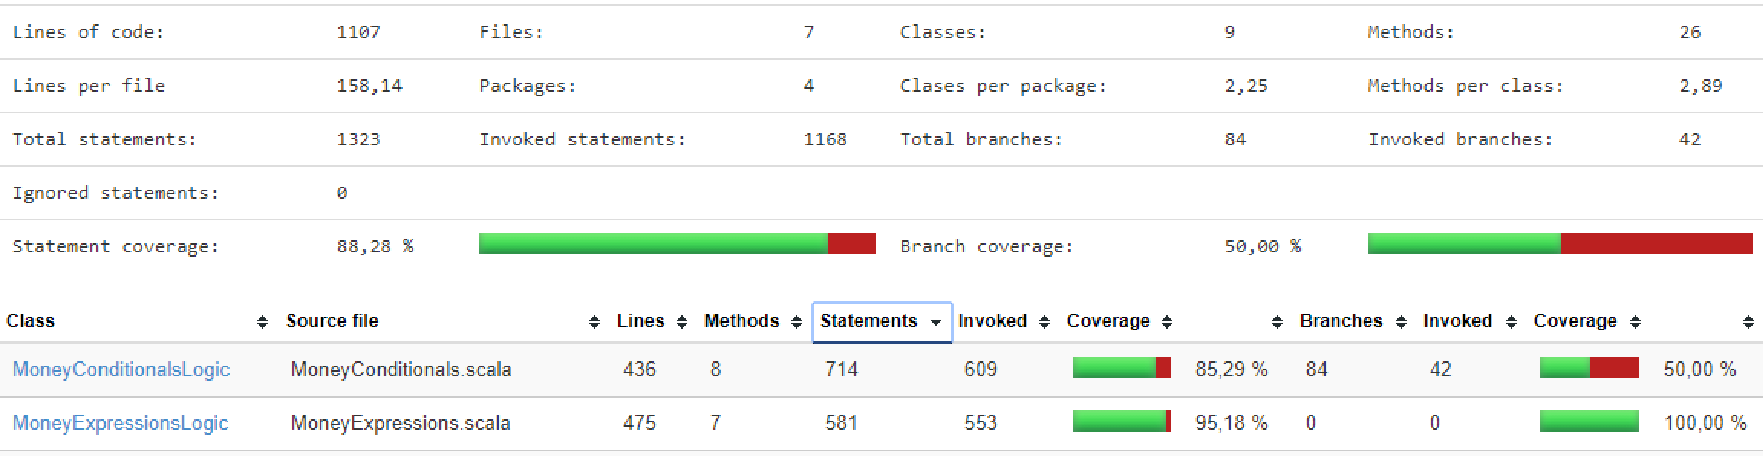
\includegraphics[width=\linewidth]{figures/eval_e3}
%}
\caption{Test coverage report of the third experiment}
\label{fig:experiment3_eval_e3}
\centering
\end{figure}
\FloatBarrier\noindent
% End figure
%\pinfo{Branch coverage still 50\%}
The branch coverage is still reported to be 50\%, while the number of branches
has been increased. This is correct, as the additional properties are using the
implication symbol, which is being translated to if-else statements. This
introduces these extra branches. As described before, we do not intend to check
the else-clause but are more interested in checking the if-clause.\\
\\
% - No extra bugs found
\pinfo{No 'extra' bugs found}
Unfortunately, no additional bugs have been found in this experiment. Additional
properties were being used in this experiment compared to the other experiments,
but these did not reveal additional bugs. The implicative properties are checked
in the same way as in the second experiment, but the values are now generated
based on the preconditions of the event definitions in the \textit{Rebel}
specification.\\
\\
%   > but increased dynamicallity. We have shown that additional properties can now be added to check, without needing to update the test framework
The properties that have been added did not require changes in the value
generator anymore. Instead, these had to be defined in the \textit{Rebel}
specification and the test framework automatically determines the values for it.
This is an improvement compared to the second experiment, as there it would be
required to update the value generator whenever an implicative property is being
added. There are still some limitations on the value generator, for example, it
does not support complex expressions as preconditions. This is also not needed
for the current set of property definitions and might or might not be needed in
the future. Because of this, we leave the implementation for supporting complex
expressions in the value generation as future work.

% % % % % % % % % % % % % % % % % % % % % % % % % % % % % % % % % % % % %
% Section: Conclusion
\section{Conclusion}
This experiment focused on improving the value generation such that it is not
required to update the test framework whenever an implicative property is being
added to the \textit{Rebel} specification. The value generator now uses the
statements in the precondition block to determine the input values, which hereby
satisfy the preconditions. We have shown that this increased the dynamicallity
by adding additional property definitions. Adding these properties to the test
framework was only a matter of translating those property definitions into the
\textit{Rebel} specification.\\
\\
This experiment did not reveal extra bugs in the generator, but we have shown
that adding more property definitions does not require an update to the test
framework when it comes to implicative properties. However, there are still some
limitations when it comes to the value generation. One of the limitations is
that it does not work with complex expressions as preconditions. The value
generator will throw an exception when an expression is given that is
unsupported.

% % % % % % % % % % % % % % % % % % % % % % % % % % % % % % % % % % % % %
% Section: Threats to validity
\section{Threats to validity}
% - Implementation error in our generator. However, we generate random values every run. (unlike Z3)
% > Running multiple times might give a fault-positive. High probability this is caused by the random operation that is done on the input values. This is a threat that came forth from experiment 2, and still exists here. - (Using > or < with 0 0 0 can happen because of this)

% - Existing approaches are available too, we only checked the Z3. But SageMath or others are possibilities too. However, this requires us to make such a tool compatible with the test framework. Our own implementation has shown to work for the properties we have defined. In case of more complex properties, it might be more useful to use another tool to determine these values.

% More reliable solving. Checked but not working as expected. Which is why we did our own generator
\subsubsection{Using existing solvers}
\pinfo{BMC possibility, tested. But not working}
Existing solvers could be used to determine a certain number of input values
that satisfy the preconditions. Since the \textit{Rebel} toolchain already makes
use of a bounded model checker to check a specification, this could be used to
translate an expression and retrieve values for which the condition holds.\\
\\
\pinfo{Checked using Z3, but returns same values all the time}
We have looked into this, by using the \textit{Z3} solver. However, the solver
always returns the same number when executing it multiple times. Which means
that the 100 values that we would ask from the generator, will be exactly the
same. A workaround would be to then add the number that was received earlier as
an additional constraint, such that 100 unique values are being retrieved. But
the problem still remains, as executing the same script multiple times will
result in the same values. Another possibility would be to change the seed of
the random generator that is being used to generate the values, resulting in
different values, however, then a random seed should be used each time the
solver is being run to make the generated values unique. In order to integrate
the solver with the test framework, the value generator has to be changed.\\
\\
An update to the value generator is required anyway to determine the input
values based on the preconditions. In addition, some existing examples to check
a \textit{Rebel} specification already take up some time. Which is probably
related to the translations that have to be done and actually running the
solver. We have not measured the exact duration of each step in this case, but
we expect that generating 100 random input values by using this approach
requires some time. Resulting in a huge run time increase for the test
framework.\\
\\
Other solvers might work better for this approach, but these still require an
update to the values generation part of the test framework to integrate with
such solvers.


%
%\pinfo{Other possibilities, future work}
%There are other solvers available too, or other methods to generate values that
%match the condition. It would be useful to make the test framework more dynamic
%when such properties are being used.

% % % % % % % % % % % % % % % % % % % % % % % % % % % % % % % % % % % % %
% Chapter: Discussion
% % % % % % % % % % % % % % % % % % % % % % % % % % % % % % % % % % % % %
\chapter{Discussion}
\label{cpt:discussion}
In this chapter we discuss the sub research questions.

% % % % % % % % % % % % % % % % % % % % % % % % % % % % % % % % % % % % %
% RQ 1: Which properties
\subsection*{RQ 1: \rqOne{}}
There were no existing properties defined for \textit{Rebel} that were expected
to hold. We have defined many properties for \textit{Rebel}. With the focus on
the \textit{Money} type, which is considered the most important type for a
bank.\\
\\
Many properties have been defined, but are these all the properties? Is each
definition correct? Some properties might be considered incorrect or overlapping
with others. We have seen this with the definition of \textit{division} that was
incorrect, which was encountered in the second experiment. In the
third experiment the property definitions for \textit{division} have been
updated. Additionally, extra properties were added to the list for the third
experiment, \textit{additivity}, \textit{subtraction} and
\textit{multiplication}. This showed how additional properties could be added to
the test framework to test the generator. In case of incorrect, missing or
overlapping property definitions, the current set of property definitions could
be updated as we have done with the third experiment. There can be many
combinations among the different types of \textit{Rebel} and the supported
operators. Therefore, the set of properties that we have defined in
\autoref{cpt:properties} is not the complete set of expected properties in
\textit{Rebel}.\\
\\
Each property definition is defined as an expression, the test framework is
currently limited to checking the generator on these kind of properties. We can also
think of other properties that should hold in \textit{Rebel}. For example, the
behaviour of sync block: what are the properties of the sync block in
\textit{Rebel}? Can these be described in a \textit{Rebel} specification? If so,
the current test framework would not support that definition yet because it can
currently only cope with expression-based properties.

% % % % % % % % % % % % % % % % % % % % % % % % % % % % % % % % % % % % %
% RQ 2: How we test
\subsection*{RQ 2: \rqTwo{}}
We have described a way how the generator can be tested by using property-based
testing. In order to check the generator, a \textit{Rebel} specification is
created containing the property definitions. This specification is used by
the test framework to generate tests and run these tests against the generated
system.\\
\\
The initial version of the test framework used random values to test each property. The first experiment showed that this doesn't work for the implicative properties. The if-clause of these implicative properties were not being triggered when using random values. In the second experiment the test framework was improved. The input values where determined such that the condition of the implicative property was being satisfied. Additionally, these values were being mutated by a random operation, to keep the randomness of the input values. This improvement to the test framework revealed some incorrect property definitions. Also, the implementation of how the input values were determined was not very dynamic. Because every time an implicative property was being added to the specification, an update was required to the test framework.\\
\\
In the third experiment the input values were determined in a more dynamic way, by using the preconditions to determine the input values. This requires a property definition to define its preconditions. As a result, it was not required to update the test framework when implicative properties were being added. This is shown in the third experiment.\\
\\
We evaluated the test framework in each experiment by looking at the test coverage and the number of bugs that have been detected. The coverage details showed that in the first experiment the if-clause of the implicative properties was not being triggered. Which lead to an improved version in the second and third experiment. Furthermore the branch coverage reported a consistent 50\% over the second and third experiment, which is caused by the implicative properties. The else-clause is not being tested, but that is also not the intention of that property.\\
\\
The overall test coverage for each experiment was roughly the same (87.80\%, 88.87\% and 88.28\%). This shows that despite of the improvements made to the test framework, the test coverage did not change. However, each experiment is different, some of the differences have an impact on the coverage results:
\begin{itemize}
  \item The first experiment used random input values for each property. The else-clause of the implicative properties were defined as \code{true}, resulting that each implicative property was considered correct.
  \item In the second experiment the else-clause of the implicative properties were set to \code{false}. The input values are generated such that these satisfy the condition of the if-clause. These values are also being mutated when running the test, to keep the actual values random.
  \item During the second experiment a fixed version of the generator was being used. This version contains fixes for the issues that were related to the \textit{Money} type. The coverage has been determined with the use of the fixed version of the generator.
  \item In the third experiment some incorrectly defined properties were updated and additional properties have been added.
  \item Note that the test framework has been updated throughout the experiments. Meaning that the third experiment contains the changes of the second experiment.
\end{itemize}
The test coverage of the first experiment would be considerably lower in case the else-clause of the implicative properties would be \code{false}. This would result in that every test concerning an implicative property would fail. Although the result of this would find many false-positives, because it just returns \textit{false} in its definition.\\
\\
The test coverage over the second and third experiment are roughly the same (only 0.59\% difference). The third experiment tested 17 more properties than the second experiment. This shows that adding additional properties does not have much impact on the test coverage. The additional properties are being checked automatically by the test framework because these properties are defined in the \textit{Rebel} specification.

% % % % % % % % % % % % % % % % % % % % % % % % % % % % % % % % % % % % %
% RQ 3: Number and kind of bugs
\subsection*{RQ 3: \rqThree{}}
Multiple bugs were found using property-based testing to check the generator.
The generator failed to satisfy a total of 8 properties that we have defined.
Some properties triggered different kind of bugs. We can categorize the bugs found as follows:
\begin{description}
  \item[~~~~Precision errors:] Errors causing an unexpected outcome value when using calculations.
  \item[~~~~Overflow/underflow errors:] Errors happening because of a value limit that has been reached on specific types.
  \item[~~~~Compilation errors:] Errors that make the generated system unable to compile, resulting that the generated system cannot be used.
\end{description}
Despite of the bugs that were found, we also found that two of the initial property definitions were incorrect. This was not found in the first experiment because of the random values. In the second experiment, this finding was the result of using a fixed version of the generator in which the precision errors related to the \textit{Money} type were fixed. This shows that some errors can hide other bugs, this is also known as finding false-negatives. We do not consider the invalid property definitions as bugs. This was not due to an error in the generator, but an error in the property definitions.\\
\\
The test framework should also be able to find other kind of bugs which did not exist in the generator that we have used. We can think of certain operations that are not correctly implemented. For example, when addition would act like subtraction. This would cause each the test case that use addition to fail.\\
\\
Also, we perhaps have missed some property definitions that would trigger more bugs in the generator. The use of other types and operators that exist in \textit{Rebel} can lead to more bugs. \textit{Rebel} also supports data structures like \textit{map} and \textit{set} which we did not cover during this thesis. Therefore we cannot conclude that the test framework would only find the kind of bugs that we found. But we can conclude that these kind of bugs can at least be found, which we have shown in the experiments.\\
\\
Below we provide a discussion about the different kind of bugs that have been found, precision errors, overflow/underflow errors and compilation errors.

\subsubsection{Precision errors}
\pinfo{Precision errors, Squants issue}
As we have seen, the \textit{Money} precision errors both occurred when using
\textit{Percentage} values as well as when using \textit{Integer} values to
operate with the \textit{Money} type. We were able to reproduce the issue
in a clean \textit{REPL} environment and concluded that the problem existed in the open-source
library, called \textit{Squants}~\cite{siteSquants2017}. This library is being used for the \textit{Money} type. In
order to solve this problem, we created an issue on
\textit{Github}\footnote{https://github.com/typelevel/squants/issues/265}
related to the precision problems on the \textit{Money} type. A contributor
responded and fixed the issue within a day, the change will be included in the
next version of the library (1.4).\\
\\
The generator should be updated to use this version of the library in order to
fix these precision errors. This is what has been done in the second experiment,
where we use the fixed version of the generator. So would updating the library
fix all the precision errors that have been found? No, in the first experiment
one of the precision errors found was being caused by multiplying a
\textit{Percentage} with an \textit{Integer}. This precision error is not
related to the precision errors when using the \textit{Money} type and still
remains to exist in the generator. There might be more precision errors when
using the generator, but then we did not define properties for these cases and
thus did not trigger those. Thus, adding more property definitions might lead to
more bugs, including precision errors.

\subsubsection{Overflow/underflow errors}
\pinfo{Overflow/underflow errors, discussion and unclear definition}
The overflow/underflow errors are caused by using the \textit{Integer} type. On
one hand, this could be prevented by checking the
operations beforehand for overflow errors. On the other hand, this could be the
expected behaviour when an \textit{Integer} is being used in \textit{Rebel}. As
\textit{Integers} are known have such limits that are also dependent on the
platform the application is run~\cite{wang2009intscope}. However, in
\textit{Rebel} there is currently no other type that can be used to hold a
bigger number. For example in \textit{Java} there is \textit{Long} for a larger
number or \textit{BigDecimal} for even bigger numbers. This would mean that
\textit{Rebel} does not support such big numbers or that a custom type must be used
for this. Although \textit{Rebel} does support custom types, the generator does
not support custom types yet. Meaning that custom types will not work with the
current implementation.\\
\\
Considering that \textit{Rebel} does not provide another type for
bigger numbers, we conclude that the \textit{Integer} type should also
hold bigger numbers. In this case, \textit{Integer} is being used to represent a
number value in \textit{Rebel}. Since the specification is about banking
products and it probably could happen that a big number is needed. After all, we
cannot know this for sure, as \textit{Rebel} does not provide a specification
yet of each of type in \textit{Rebel}. Maybe it is not needed or required to
support bigger numbers than an integer, resulting in that our conclusion is
incorrect. But what would be the minimum and maximum value it can hold then? Would it be the
value of a 32 bit \textit{Integer} or a 64 bit \textit{Integer}. In case our conclusion is
incorrect, this should be defined too. The property definition could be updated
to describe the actual bounds of the input values.

\subsubsection{Compilation errors}
\pinfo{Compilation error, Squants issue}
In the first experiment, the test framework was initially being terminated because of a
compilation error. Although one assumption was that the generated system should
be able to compile, another assumption was that the specification was
consistent. The specification containing all the properties is consistent,
as \textit{Rebel} did not report any syntactic or semantic errors with the type
checker. Because of this, it was expected that the generated system could
compile and run.\\
\\
The test framework is able to find such compilation errors, as we have seen in the first experiment. However, the test framework cannot proceed with running the generated tests in this case, thus hiding other bugs that can exist. The test framework does not specifically check for compile errors and whether these are expected or not. This is out of the scope of this thesis, because there can be many causes of compilation errors in the generated system and detecting the actual causes of those is hard, if not impossible.\\
\\
The cause of the compilation error we found in the first experiment was an implementation error in the open-source library that is being used for the \textit{Money} type called \textit{Squants}~\cite{siteSquants2017}. We
created a \textit{Github} issue\footnote{https://github.com/typelevel/squants/issues/281} describing this problem. When this issue has been fixed, the generator should be updated in order to fix this compilation error. Since this issue has not been fixed during this thesis, we temporarily disabled the property causing this problem.

% Advice?
% To think of: Where there some things encountered during the project, which might require attention, but haven't or won't be thoroughly tested with this approach. Or do some additions cover these?
% > Squants
%	- Some bugs, maybe there are more in there
% 	- Snapshot release unavailable for some time? (1.4.0-SNAPSHOT was not reachable, had to compile it ourselves)

% % % % % % % % % % % % % % % % % % % % % % % % % % % % % % % % % % % % %
% Chapter: Conclusion
% % % % % % % % % % % % % % % % % % % % % % % % % % % % % % % % % % % % %
\chapter{Conclusion}
\label{cpt:conclusion}
% Summary
In this thesis, we have shown a way how the generator can be tested by using property-based testing. This is done by generating tests based on the \textit{Rebel} specification and making use of the generator to generate the tests. The \textit{Rebel} specification is build up based on a set of defined properties of \textit{Rebel}. These property definitions were not defined earlier, thus we defined many expected properties in \textit{Rebel}.\\
\\
With test framework we have found some bugs in the generated system that were unknown before. This proves that this approach already worked to identify some problems in the generator that were not known before. Additionally, we contributed to an open-source library called \textit{Squants}, by issuing two reports of bugs that existed in the library.\\
\\
% Research questions
% Answer main research question
To answer the main research question, we defined and answered the three sub research questions, which have been discussed in \autoref{cpt:discussion}. The main research question was as follows:
\begin{quote}
\rqMain
\end{quote}
A \textit{Rebel} specification is created from the defined properties. Next, the existing generator is being used to generate the generated system and to translate the properties (in the \textit{Rebel} specification) to test cases. When running the test framework, we found some errors by using the generated system. Additionally, we were able to detect a compilation error and incorrectly translated formulas.\\
\\
We conclude that, by using this approach, the semantics of the generated code can be checked automatically on whether it satisfies the defined properties. With this approach, we have found bugs in the generated code that were unknown before.

% % % % % % % % % % % % % % % % % % % % % % % % % % % % % % % % % % % % %
% Section: Future work
\section{Future work}
% Multi VM testing, specify sync properties, can test with multi JVM testing etc. Sources > future work

\subsubsection{Complete property definitions}
\pinfo{Full definitions for Rebel}
In this thesis, we defined some properties on the \textit{Rebel} language,
which we consider to hold when using \textit{Rebel}. This list of property
definitions on \textit{Rebel} is not complete, there can be many more properties
and there are other types available in \textit{Rebel} which we did not cover.
Defining these and adding them to the set of property definitions is left as
future work.

\subsubsection{Values generation by using solvers}
\pinfo{Current value generation limitations}
The current value generation works for the properties that we defined throughout this thesis. When additional properties are being added, the value generator might or might not have to be updated. This depends on what preconditions have to be parsed for that property and whether the current implementation supports these operations.\\% As described, the current implementation has some limitations. It does not support expressions that are using different operators or that use expressions on both the left-hand and right-hand side (expressions here means non-literals or variables, but a combination of operators and literals/variables).\\
\\
\pinfo{Other tools possible}
Another way how the value generator could work is to use some tools to determine the random values. As we have discussed in \autoref{cpt:experiment3}, the SMT solver would theoratically be an option. But in our attempts this resulted in having the same input values every time the test framework is run. To counter this problem, other solvers might be more useful to implement this behaviour, such as \textit{SageMath}~\cite{siteSageMath2017}. \textit{SageMath} can parse expressions and determine the conditions to which each variable in the expression should hold. When using this, it would mean that the value generator has to be modified such that it integrates with this tool. Another approach could be used for this too, such as concolic testing~\cite{sen2006cute} to determine the input values. We did not use this in this thesis, due to time constraints.
% Maybe there are some QuickCheck ports that do this already for some languages?

\subsubsection{Multiple generators}
\pinfo{Only one, support for more could be added}
Throughout this thesis, we have only tested the Scala/Akka generator which is
developed by \textit{ING}. Since there are more generators available, the test
framework can be improved such that it is
compatible with the other systems that can be generated by using one of the
other generators that are available within \textit{ING}. By doing this, the same
property definitions can be tested on different kind of generated systems. This
can be used to detect inequalities among the generated systems. Although the properties will remain the same in this case, generating the test suite requires some modifications for each generator.\\
\\
\textit{Templating} is used to generate the test cases. The way how the tests should be written down depends on the generated system. When a generated system uses a different setup or is written in another language then \textit{Scala}, an update is needed for this part of the test framework. The other parts of the test framework can be reused, as the test framework also uses the generator from which the generated system is created.

\subsubsection{Mutation testing}
Another metric to evaluate the effectiveness of the test framework would be to use
mutation testing. The mutation coverage could be used to measure how
effective the test framework would be (the number of mutants created and the
number of killed mutants). Unfortunately, there is currently a limited support
for mutation testing for \textit{Scala} systems. \textit{PIT} for example, cannot meaningfully
mutate \textit{Scala} code~\cite{siteSbtPit2017}. Because of this, we did not
use this as metric to evaluate the test framework.\\
\\
\textit{Scala} compiles to \textit{Java} bytecode, mutating on bytecode level
could be used too. However, some mutants might not be relevant in that the
modifications would not affect the implementation, which can lead to
false-positives.

\subsubsection{Other components}
Besides completing the set of property definitions, the test framework could also be extended such that it
can also support property definitions concerning other components of the system. Such as the sync block
definitions, which defines actions that should happen synchronously. Or performance
measures when interacting with data in the system. Currently, such components
are not being tested and are unsupported, while these
components are also important for the bank. This is left as future work.\\
\\
It might not be possible to check each and every component
by using this approach. For example, it might be unable to check how
multiple generated systems would integrate with each other and if this is done
correctly. The generated system is configured to work with multiple
distributions of the system, but is not being tested thoroughly yet.

% Ultimately, as last
%\subsubsection{Properties based on type checker}
%\pinfo{Generating properties based on type checker}
%\textit{Rebel} contains a type checker, which is able to determine exactly
%which operations are supported by using certain combinations of operators and
%types. This could be used to automatically generate the property specifications
%in \textit{Rebel} based on whether a type supports certain operations that are
%required for the property. For example, if \textit{Percentage} supports
%addition, the properties for \textit{additivity}, \textit{associativeAddition}
%and \textit{commutativeAddition} can be generated based on this rule.\\
%\\
%A map of all operations and all existing types could be created. Next, each
%combination can be tested against the type checker. If the type checker an
%expression as correct, the event definition for some properties could be
%be generated. Although this might result in many event definitions,
%with a possible overlap between them, it could be a way to automatically
%generate the specification containing the definitions. This assumes that the type
%checker does the right thing, which is a threat to this approach. This
%can also lead to more compilation errors in the generated system. Nevertheless,
%it can make it more dynamic when a new type is being added to the \textit{Rebel}
%language.

% % % % % % % % % % % % % % % % % % % % % % % % % % % % % % % % % % % % %
% Chapter: Bibliography
% % % % % % % % % % % % % % % % % % % % % % % % % % % % % % % % % % % % %
%{%\tiny
%\bibliographystyle{alphaurl}
\bibliographystyle{ieeetr}
\bibliography{thesis}
%}

% % % % % % % % % % % % % % % % % % % % % % % % % % % % % % % % % % % % %
% Chapter: Appendices
% % % % % % % % % % % % % % % % % % % % % % % % % % % % % % % % % % % % %
\appendix
% % % % % % % % % % % % % % % % % % % % % % % % % % % % % % % % % % % % %
% Section: Appendix I: Property definitions of Rebel in Rebel
\chapter{Property definitions in Rebel}
\label{app:a_event_definitions}
% Listing
\begin{sourcecode}[!ht]
\begin{lstlisting}[language=Rebel]
event reflexiveEquality(x: Money) {
    postconditions {
       new this.result == ( x == x );
    }
}

event reflexiveInequalityLET(x: Money) {
    postconditions {
       new this.result == ( x <= x );
    }
}

event reflexiveInequalityGET(x: Money) {
    postconditions {
       new this.result == ( x >= x );
    }
}

event symmetric(x: Money, y:Money) {
    postconditions {
       new this.result == ( (x == y) ? y == x : True );
    }
}

event transitiveEquality(x: Money, y: Money, z: Money) {
    postconditions {
       new this.result == ( (x == y && y == z) ? x == z : True );
    }
}

event transitiveInequalityLT(x: Money, y: Money, z: Money) {
    postconditions {
       new this.result == ( (x < y && y < z) ? x < z : True );
    }
}

event transitiveInequalityGT(x: Money, y: Money, z: Money) {
    postconditions {
       new this.result == ( (x > y && y > z) ? x > z : True );
    }
}
\end{lstlisting}
\caption{The property definitions as \textit{Rebel} specification}
\end{sourcecode}
\FloatBarrier\noindent
% End listing
% Listing
\begin{sourcecode}[!ht]
\begin{lstlisting}[language=Rebel]
event transitiveInequalityLET(x: Money, y: Money, z: Money) {
    postconditions {
       new this.result == ( (x <= y && y <= z) ? x <= z : True );
    }
}

event transitiveInequalityGET(x: Money, y: Money, z: Money) {
    postconditions {
       new this.result == ( (x >= y && y >= z) ? x >= z : True );
    }
}

event additive(x: Money, y: Money, z: Money) {
    postconditions {
         new this.result == ( (x==y) ? x+z == y+z : True );
    }
}

event additive4params(x: Money, y: Money, z: Money, a: Money) {
    postconditions {
        new this.result == ( (x == y && z == a) ? x+z == y+a : True );
    }
}

event commutativeAddition(x: Money, y: Money) {
    postconditions {
        new this.result == ( x+y == y+x );
    }
}

event commutativeMultiplicationInteger1(x: Integer, y: Money) {
    postconditions {
        new this.result == ( x*y == y*x );
    }
}

event commutativeMultiplicationInteger2(x: Money, y: Integer) {
    postconditions {
        new this.result == ( x*y == y*x );
    }
}

event commutativeMultiplicationPercentage1(x: Percentage, y: Money) {
    postconditions {
        new this.result == ( x*y == y*x );
    }
}

event commutativeMultiplicationPercentage2(x: Money, y: Percentage) {
    postconditions {
        new this.result == ( x*y == y*x );
    }
}

event associativeAddition(x: Money, y: Money, z: Money) {
    postconditions {
        new this.result == ( (x+y)+z == x+(y+z) );
    }
}

event associativeMultiplicationInteger1(x: Integer, y: Integer, z: Money) {
    postconditions {
        new this.result == ( (x*y)*z == x*(y*z) );
    }
}
\end{lstlisting}
\caption{The property definitions as \textit{Rebel} specification (continued)}
\end{sourcecode}
\FloatBarrier\noindent
% End listing
% Listing
\begin{sourcecode}[!ht]
\begin{lstlisting}[language=Rebel]
event associativeMultiplicationInteger2(x: Money, y: Integer, z: Integer) {
    postconditions {
        new this.result == ( (x*y)*z == x*(y*z) );
    }
}

event associativeMultiplicationPercentage1(x: Money, y: Percentage, z: Integer) {
    postconditions {
        new this.result == ( (x*y)*z == x*(y*z) );
    }
}

event associativeMultiplicationPercentage2(x: Integer, y: Money, z: Percentage) {
    postconditions {
        new this.result == ( (x*y)*z == x*(y*z) );
    }
}

event distributiveInteger1(x: Money, y: Integer, z: Integer) {
    postconditions {
        new this.result == ( x*(y+z) == x*y + x*z );
    }
}

event distributiveInteger2(x: Integer, y: Money, z: Money) {
    postconditions {
        new this.result == ( (y+z)*x == y*x + z*x );
    }
}

event distributivePercentage1(x: Percentage, y: Money, z: Money) {
    postconditions {
        new this.result == ( x*(y+z) == x*y + x*z );
    }
}

event distributivePercentage2(x: Percentage, y: Money, z: Money) {
    postconditions {
        new this.result == ( (y+z)*x == y*x + z*x );
    }
}

event additiveIdentity1(x: Money) {
    postconditions {
        new this.result == ( x + EUR 0.00 == x );
    }
}

event additiveIdentity2(x: Money) {
    postconditions {
        new this.result == ( EUR 0.00 + x == x );
    }
}

event multiplicativeIdentity1(x: Money) {
    postconditions {
        new this.result == ( x*1 == x );
    }
}
event multiplicativeIdentity2(x: Money) {
    postconditions {
        new this.result == ( 1*x == x );
    }
}
\end{lstlisting}
\caption{The property definitions as \textit{Rebel} specification (continued)}
\end{sourcecode}
\FloatBarrier\noindent
% End listing

% Listing
\begin{sourcecode}[!ht]
\begin{lstlisting}[language=Rebel]
event additiveInverse1(x: Money) {
    postconditions {
        new this.result == ( x+(-x) == EUR 0.00 );
    }
}

event additiveInverse2(x: Money) {
    postconditions {
        new this.result == ( (-x)+x == EUR 0.00 );
    }
}

event antisymmetryLET(x: Money, y: Money) {
    postconditions {
        new this.result == ( (x <= y && y <= x) ? x == y : True );
    }
}

event antisymmetryGET(x: Money, y: Money) {
    postconditions {
        new this.result == ( (x >= y && y >= x) ? x == y : True );
    }
}

event division1(x: Money, y: Integer, z: Money) {
    postconditions {
        new this.result == ( (x*y == z) ? (x == z/y) : True );
    }
}

event division2(x: Money, y: Integer, z: Money) {
    postconditions {
        new this.result == ( (x == z*y) ? (x/y == z) : True );
    }
}

event multiplicativeZeroProperty1(x: Money) {
    postconditions {
        new this.result == ( x*0 == EUR 0.00 );
    }
}

event multiplicativeZeroProperty2(x: Money) {
    postconditions {
        new this.result == ( 0*x == EUR 0.00 );
    }
}

event anticommutativity(x: Money, y: Money) {
    postconditions {
        new this.result == ( x-y == -(y-x) );
    }
}

event nonassociativity(x: Money, y: Money, z: Money) {
    postconditions {
        new this.result == ( (x-y)-z != x-(y-z) );
    }
}

event trichotomy(x: Money, y: Money) {
    postconditions {
        new this.result == ( x < y || x == y || x > y );
    }
}
\end{lstlisting}
\caption{The property definitions as \textit{Rebel} specification (continued)}
\end{sourcecode}
\FloatBarrier\noindent
% End listing

% % % % % % % % % % % % % % % % % % % % % % % % % % % % % % % % % % % % %
% Section: Appendix II:
\chapter{Additional property definitions}
\label{app:b_event_definitions_additional}
% Listing
\begin{sourcecode}[!ht]
\begin{lstlisting}[language=Rebel]
event divisionEquality1(x: Money, y: Integer, z: Money) {
    preconditions {
        round((x*y)) == round((z));
    }
    postconditions {
        new this.result == ( (round(x*y) == round(z)) ? (round(x) == round(z/y)) : False );
    }
}

event divisionEquality2(x: Money, y: Integer, z: Money) {
    preconditions {
        round((x)) == round((z*y));
    }
    postconditions {
        new this.result == ( (round(x) == round(z*y)) ? (round(x/y) == round(z)) : False );
    }
}

event divisionEquality3(x: Money, y: Money, z: Integer) {
    preconditions {
        x == y;
        z != 0;
    }
    postconditions {
        new this.result == ( (x == y && z != 0) ? (x/z == y/z) : False );
    }
}

event divisionInequalityLT1(x: Money, y: Money, z: Integer) {
    preconditions {
        x < y;
        z > 0;
    }
    postconditions {
        new this.result == ( (x < y && z > 0) ? (x/z < y/z) : False );
    }
}
\end{lstlisting}
\caption{Additional property definitions as \textit{Rebel} specification}
\end{sourcecode}
\FloatBarrier\noindent
% End listing

% Listing
\begin{sourcecode}[!ht]
\begin{lstlisting}[language=Rebel]
event divisionInequalityLT2(x: Money, y: Money, z: Integer) {
    preconditions {
        x < y;
        z < 0;
    }
    postconditions {
        new this.result == ( (x < y && z < 0) ? (x/z > y/z) : False );
    }
}

event divisionInequalityLGT1(x: Money, y: Money, z: Integer) {
    preconditions {
        x > y;
        z > 0;
    }
    postconditions {
        new this.result == ( (x > y && z > 0) ? (x/z > y/z) : False );
    }
}

event divisionInequalityLGT2(x: Money, y: Money, z: Integer) {
    preconditions {
        x > y;
        z < 0;
    }
    postconditions {
        new this.result == ( (x > y && z < 0) ? (x/z < y/z) : False );
    }
}

event additiveEquality(x: Money, y: Money, z: Money) {
    preconditions {
        x == y;
    }
    postconditions {
         new this.result == ( (x==y) ? x+z == y+z : False );
    }
}

event additiveEquality4params(x: Money, y: Money, z: Money, a: Money) {
    preconditions {
        x == y;
        z == a;
    }
    postconditions {
        new this.result == ( (x == y && z == a) ? x+z == y+a : False );
    }
}

event additiveInequalityLT(x: Money, y: Money, z: Money) {
    preconditions {
        x < y;
    }
    postconditions {
         new this.result == ( (x<y) ? x+z < y+z : False );
    }
}

event additiveInequalityGT(x: Money, y: Money, z: Money) {
    preconditions {
        x > y;
    }
    postconditions {
         new this.result == ( (x>y) ? x+z > y+z : False );
    }
}
\end{lstlisting}
\caption{Additional property definitions as \textit{Rebel} specification (continued)}
\end{sourcecode}
\FloatBarrier\noindent
% End listing

% Listing
\begin{sourcecode}[!ht]
\begin{lstlisting}[language=Rebel]
event subtractiveEquality(x: Money, y: Money, z: Money) {
    preconditions {
        x == y;
    }
    postconditions {
        new this.result == ( (x==y) ? (x-z == y-z) : False );
    }
}

event subtractiveInequalityLT(x: Money, y: Money, z: Money) {
    preconditions {
        x < y;
    }
    postconditions {
        new this.result == ( (x<y) ? (x-z < y-z) : False );
    }
}

event subtractiveInequalityGT(x: Money, y: Money, z: Money) {
    preconditions {
        x > y;
    }
    postconditions {
        new this.result == ( (x>y) ? (x-z > y-z) : False );
    }
}

event multiplicativeEquality(x: Money, y: Money, z: Integer) {
    preconditions {
        x == y;
    }
    postconditions {
        new this.result == ( (x==y) ? (x*z == y*z) : False );
    }
}

event multiplicativeInequalityLT1(x: Money, y: Money, z: Integer) {
    preconditions {
        x < y;
        z > 0;
    }
    postconditions {
        new this.result == ( (x<y && z > 0) ? (x*z < y*z) : False );
    }
}

event multiplicativeInequalityLT2(x: Money, y: Money, z: Integer) {
    preconditions {
        x < y;
        z < 0;
    }
    postconditions {
        new this.result == ( (x<y && z < 0) ? (x*z > y*z) : False );
    }
}

event multiplicativeInequalityGT1(x: Money, y: Money, z: Integer) {
    preconditions {
        x > y;
        z > 0;
    }
    postconditions {
        new this.result == ( (x>y && z > 0) ? (x*z > y*z) : False );
    }
}
\end{lstlisting}
\caption{Additional property definitions as \textit{Rebel} specification (continued)}
\end{sourcecode}
\FloatBarrier\noindent
% End listing

% Listing
\begin{sourcecode}[!ht]
\begin{lstlisting}[language=Rebel]
event multiplicativeInequalityGT2(x: Money, y: Money, z: Integer) {
    preconditions {
        x > y;
        z < 0;
    }
    postconditions {
        new this.result == ( (x>y && z < 0) ? (x*z < y*z) : False );
    }
}
\end{lstlisting}
\caption{Additional property definitions as \textit{Rebel} specification (continued)}
\end{sourcecode}
\FloatBarrier\noindent
% End listing


\end{document}


% % % % % % % % % % % % % % % % % % % % % % % % % % % % % % % %
% Possible further improvements (TODO's):
% - Background: Rebel Keller source for labeled transition system
% - Test mechanics: Also define efficiency? Not yet, requires many changes and rerunning is all again.
% - Properties: Also describe percentage? Not yet, requires defining, reasoning, and running it all again. And possibly updating evaluations too
